% Options for packages loaded elsewhere
\PassOptionsToPackage{unicode}{hyperref}
\PassOptionsToPackage{hyphens}{url}
%
\documentclass[
]{book}
\usepackage{amsmath,amssymb}
\usepackage{iftex}
\ifPDFTeX
  \usepackage[T1]{fontenc}
  \usepackage[utf8]{inputenc}
  \usepackage{textcomp} % provide euro and other symbols
\else % if luatex or xetex
  \usepackage{unicode-math} % this also loads fontspec
  \defaultfontfeatures{Scale=MatchLowercase}
  \defaultfontfeatures[\rmfamily]{Ligatures=TeX,Scale=1}
\fi
\usepackage{lmodern}
\ifPDFTeX\else
  % xetex/luatex font selection
\fi
% Use upquote if available, for straight quotes in verbatim environments
\IfFileExists{upquote.sty}{\usepackage{upquote}}{}
\IfFileExists{microtype.sty}{% use microtype if available
  \usepackage[]{microtype}
  \UseMicrotypeSet[protrusion]{basicmath} % disable protrusion for tt fonts
}{}
\makeatletter
\@ifundefined{KOMAClassName}{% if non-KOMA class
  \IfFileExists{parskip.sty}{%
    \usepackage{parskip}
  }{% else
    \setlength{\parindent}{0pt}
    \setlength{\parskip}{6pt plus 2pt minus 1pt}}
}{% if KOMA class
  \KOMAoptions{parskip=half}}
\makeatother
\usepackage{xcolor}
\usepackage{color}
\usepackage{fancyvrb}
\newcommand{\VerbBar}{|}
\newcommand{\VERB}{\Verb[commandchars=\\\{\}]}
\DefineVerbatimEnvironment{Highlighting}{Verbatim}{commandchars=\\\{\}}
% Add ',fontsize=\small' for more characters per line
\usepackage{framed}
\definecolor{shadecolor}{RGB}{248,248,248}
\newenvironment{Shaded}{\begin{snugshade}}{\end{snugshade}}
\newcommand{\AlertTok}[1]{\textcolor[rgb]{0.94,0.16,0.16}{#1}}
\newcommand{\AnnotationTok}[1]{\textcolor[rgb]{0.56,0.35,0.01}{\textbf{\textit{#1}}}}
\newcommand{\AttributeTok}[1]{\textcolor[rgb]{0.13,0.29,0.53}{#1}}
\newcommand{\BaseNTok}[1]{\textcolor[rgb]{0.00,0.00,0.81}{#1}}
\newcommand{\BuiltInTok}[1]{#1}
\newcommand{\CharTok}[1]{\textcolor[rgb]{0.31,0.60,0.02}{#1}}
\newcommand{\CommentTok}[1]{\textcolor[rgb]{0.56,0.35,0.01}{\textit{#1}}}
\newcommand{\CommentVarTok}[1]{\textcolor[rgb]{0.56,0.35,0.01}{\textbf{\textit{#1}}}}
\newcommand{\ConstantTok}[1]{\textcolor[rgb]{0.56,0.35,0.01}{#1}}
\newcommand{\ControlFlowTok}[1]{\textcolor[rgb]{0.13,0.29,0.53}{\textbf{#1}}}
\newcommand{\DataTypeTok}[1]{\textcolor[rgb]{0.13,0.29,0.53}{#1}}
\newcommand{\DecValTok}[1]{\textcolor[rgb]{0.00,0.00,0.81}{#1}}
\newcommand{\DocumentationTok}[1]{\textcolor[rgb]{0.56,0.35,0.01}{\textbf{\textit{#1}}}}
\newcommand{\ErrorTok}[1]{\textcolor[rgb]{0.64,0.00,0.00}{\textbf{#1}}}
\newcommand{\ExtensionTok}[1]{#1}
\newcommand{\FloatTok}[1]{\textcolor[rgb]{0.00,0.00,0.81}{#1}}
\newcommand{\FunctionTok}[1]{\textcolor[rgb]{0.13,0.29,0.53}{\textbf{#1}}}
\newcommand{\ImportTok}[1]{#1}
\newcommand{\InformationTok}[1]{\textcolor[rgb]{0.56,0.35,0.01}{\textbf{\textit{#1}}}}
\newcommand{\KeywordTok}[1]{\textcolor[rgb]{0.13,0.29,0.53}{\textbf{#1}}}
\newcommand{\NormalTok}[1]{#1}
\newcommand{\OperatorTok}[1]{\textcolor[rgb]{0.81,0.36,0.00}{\textbf{#1}}}
\newcommand{\OtherTok}[1]{\textcolor[rgb]{0.56,0.35,0.01}{#1}}
\newcommand{\PreprocessorTok}[1]{\textcolor[rgb]{0.56,0.35,0.01}{\textit{#1}}}
\newcommand{\RegionMarkerTok}[1]{#1}
\newcommand{\SpecialCharTok}[1]{\textcolor[rgb]{0.81,0.36,0.00}{\textbf{#1}}}
\newcommand{\SpecialStringTok}[1]{\textcolor[rgb]{0.31,0.60,0.02}{#1}}
\newcommand{\StringTok}[1]{\textcolor[rgb]{0.31,0.60,0.02}{#1}}
\newcommand{\VariableTok}[1]{\textcolor[rgb]{0.00,0.00,0.00}{#1}}
\newcommand{\VerbatimStringTok}[1]{\textcolor[rgb]{0.31,0.60,0.02}{#1}}
\newcommand{\WarningTok}[1]{\textcolor[rgb]{0.56,0.35,0.01}{\textbf{\textit{#1}}}}
\usepackage{longtable,booktabs,array}
\usepackage{calc} % for calculating minipage widths
% Correct order of tables after \paragraph or \subparagraph
\usepackage{etoolbox}
\makeatletter
\patchcmd\longtable{\par}{\if@noskipsec\mbox{}\fi\par}{}{}
\makeatother
% Allow footnotes in longtable head/foot
\IfFileExists{footnotehyper.sty}{\usepackage{footnotehyper}}{\usepackage{footnote}}
\makesavenoteenv{longtable}
\usepackage{graphicx}
\makeatletter
\def\maxwidth{\ifdim\Gin@nat@width>\linewidth\linewidth\else\Gin@nat@width\fi}
\def\maxheight{\ifdim\Gin@nat@height>\textheight\textheight\else\Gin@nat@height\fi}
\makeatother
% Scale images if necessary, so that they will not overflow the page
% margins by default, and it is still possible to overwrite the defaults
% using explicit options in \includegraphics[width, height, ...]{}
\setkeys{Gin}{width=\maxwidth,height=\maxheight,keepaspectratio}
% Set default figure placement to htbp
\makeatletter
\def\fps@figure{htbp}
\makeatother
\setlength{\emergencystretch}{3em} % prevent overfull lines
\providecommand{\tightlist}{%
  \setlength{\itemsep}{0pt}\setlength{\parskip}{0pt}}
\setcounter{secnumdepth}{5}
\usepackage{booktabs}
\usepackage{booktabs}
\usepackage{longtable}
\usepackage{array}
\usepackage{multirow}
\usepackage{wrapfig}
\usepackage{float}
\usepackage{colortbl}
\usepackage{pdflscape}
\usepackage{tabu}
\usepackage{threeparttable}
\usepackage{threeparttablex}
\usepackage[normalem]{ulem}
\usepackage{makecell}
\usepackage{xcolor}
\ifLuaTeX
  \usepackage{selnolig}  % disable illegal ligatures
\fi
\usepackage[]{natbib}
\bibliographystyle{plainnat}
\IfFileExists{bookmark.sty}{\usepackage{bookmark}}{\usepackage{hyperref}}
\IfFileExists{xurl.sty}{\usepackage{xurl}}{} % add URL line breaks if available
\urlstyle{same}
\hypersetup{
  pdftitle={Bivariate Regression},
  pdfauthor={Ben Gonzalez},
  hidelinks,
  pdfcreator={LaTeX via pandoc}}

\title{Bivariate Regression}
\author{Ben Gonzalez}
\date{2023-10-06}

\usepackage{amsthm}
\newtheorem{theorem}{Theorem}[chapter]
\newtheorem{lemma}{Lemma}[chapter]
\newtheorem{corollary}{Corollary}[chapter]
\newtheorem{proposition}{Proposition}[chapter]
\newtheorem{conjecture}{Conjecture}[chapter]
\theoremstyle{definition}
\newtheorem{definition}{Definition}[chapter]
\theoremstyle{definition}
\newtheorem{example}{Example}[chapter]
\theoremstyle{definition}
\newtheorem{exercise}{Exercise}[chapter]
\theoremstyle{definition}
\newtheorem{hypothesis}{Hypothesis}[chapter]
\theoremstyle{remark}
\newtheorem*{remark}{Remark}
\newtheorem*{solution}{Solution}
\begin{document}
\maketitle

{
\setcounter{tocdepth}{1}
\tableofcontents
}
\hypertarget{about}{%
\chapter{About}\label{about}}

This is a \emph{sample} book written in \textbf{Markdown}. You can use anything that Pandoc's Markdown supports; for example, a math equation \(a^2 + b^2 = c^2\).

\hypertarget{usage}{%
\section{Usage}\label{usage}}

Each \textbf{bookdown} chapter is an .Rmd file, and each .Rmd file can contain one (and only one) chapter. A chapter \emph{must} start with a first-level heading: \texttt{\#\ A\ good\ chapter}, and can contain one (and only one) first-level heading.

Use second-level and higher headings within chapters like: \texttt{\#\#\ A\ short\ section} or \texttt{\#\#\#\ An\ even\ shorter\ section}.

The \texttt{index.Rmd} file is required, and is also your first book chapter. It will be the homepage when you render the book.

\hypertarget{render-book}{%
\section{Render book}\label{render-book}}

You can render the HTML version of this example book without changing anything:

\begin{enumerate}
\def\labelenumi{\arabic{enumi}.}
\item
  Find the \textbf{Build} pane in the RStudio IDE, and
\item
  Click on \textbf{Build Book}, then select your output format, or select ``All formats'' if you'd like to use multiple formats from the same book source files.
\end{enumerate}

Or build the book from the R console:

\begin{Shaded}
\begin{Highlighting}[]
\NormalTok{bookdown}\SpecialCharTok{::}\FunctionTok{render\_book}\NormalTok{()}
\end{Highlighting}
\end{Shaded}

To render this example to PDF as a \texttt{bookdown::pdf\_book}, you'll need to install XeLaTeX. You are recommended to install TinyTeX (which includes XeLaTeX): \url{https://yihui.org/tinytex/}.

\hypertarget{preview-book}{%
\section{Preview book}\label{preview-book}}

As you work, you may start a local server to live preview this HTML book. This preview will update as you edit the book when you save individual .Rmd files. You can start the server in a work session by using the RStudio add-in ``Preview book'', or from the R console:

\begin{Shaded}
\begin{Highlighting}[]
\NormalTok{bookdown}\SpecialCharTok{::}\FunctionTok{serve\_book}\NormalTok{()}
\end{Highlighting}
\end{Shaded}

Statistical Significance - Confidence Intervals - Effect Size

\begin{verbatim}
## 
## Attaching package: 'dplyr'
\end{verbatim}

\begin{verbatim}
## The following objects are masked from 'package:stats':
## 
##     filter, lag
\end{verbatim}

\begin{verbatim}
## The following objects are masked from 'package:base':
## 
##     intersect, setdiff, setequal, union
\end{verbatim}

\hypertarget{sample-standard-deviation-formula}{%
\subsubsection{Sample Standard Deviation Formula}\label{sample-standard-deviation-formula}}

\[\large
S\;=\;\sqrt{\frac{\sum(X\;-\;{\overline{X}})^2}{N\;-1}}
\]

\begin{Shaded}
\begin{Highlighting}[]
\NormalTok{N }\OtherTok{\textless{}{-}} \FunctionTok{length}\NormalTok{(mtcars}\SpecialCharTok{$}\NormalTok{hp)}
\NormalTok{deviations }\OtherTok{\textless{}{-}}\NormalTok{ mtcars}\SpecialCharTok{$}\NormalTok{hp}\SpecialCharTok{{-}}\FunctionTok{mean}\NormalTok{(mtcars}\SpecialCharTok{$}\NormalTok{hp)}

\NormalTok{s }\OtherTok{\textless{}{-}}\NormalTok{ deviations}\SpecialCharTok{\^{}}\DecValTok{2}

\NormalTok{m\_plus}\OtherTok{\textless{}{-}} \FunctionTok{sum}\NormalTok{(s)}\SpecialCharTok{/}\NormalTok{(N}\DecValTok{{-}1}\NormalTok{)}

\NormalTok{sd\_plus }\OtherTok{\textless{}{-}} \FunctionTok{sqrt}\NormalTok{(m\_plus)}
\FunctionTok{print}\NormalTok{(sd\_plus)}
\end{Highlighting}
\end{Shaded}

\begin{verbatim}
## [1] 68.56287
\end{verbatim}

\begin{Shaded}
\begin{Highlighting}[]
\FunctionTok{sqrt}\NormalTok{((}\FunctionTok{sum}\NormalTok{((mtcars}\SpecialCharTok{$}\NormalTok{hp}\SpecialCharTok{{-}}\FunctionTok{mean}\NormalTok{(mtcars}\SpecialCharTok{$}\NormalTok{hp))}\SpecialCharTok{\^{}}\DecValTok{2}\NormalTok{))}\SpecialCharTok{/}\NormalTok{(}\FunctionTok{length}\NormalTok{(mtcars}\SpecialCharTok{$}\NormalTok{hp)}\SpecialCharTok{{-}}\DecValTok{1}\NormalTok{))}
\end{Highlighting}
\end{Shaded}

\begin{verbatim}
## [1] 68.56287
\end{verbatim}

\begin{Shaded}
\begin{Highlighting}[]
\FunctionTok{sd}\NormalTok{(mtcars}\SpecialCharTok{$}\NormalTok{hp)}
\end{Highlighting}
\end{Shaded}

\begin{verbatim}
## [1] 68.56287
\end{verbatim}

\hypertarget{standard-error-formula}{%
\subsubsection{Standard Error Formula}\label{standard-error-formula}}

\[\large
SE\;\;=\frac{\sigma}{\sqrt{n}}
\]
\[
SE\;=Standard\;Error
\\
\sigma\;=sample\;standard\;deviation
\\
n\;=number\;of\;samples
\]

\hypertarget{how-to-calculate-the-standard-error-of-a-sample}{%
\subsubsection{How to calculate the standard error of a sample}\label{how-to-calculate-the-standard-error-of-a-sample}}

\begin{Shaded}
\begin{Highlighting}[]
\CommentTok{\#standard deviation/squareroot(n)}

\CommentTok{\# length(mtcars$hp)}
\CommentTok{\# nrow(mtcars)}

\DocumentationTok{\#\#\#Shortcut to calculate the standard error of a sample}
\DocumentationTok{\#\#\#The length function is utilized to find the number of observations in a data set}
\FunctionTok{sd}\NormalTok{(mtcars}\SpecialCharTok{$}\NormalTok{hp)}\SpecialCharTok{/}\FunctionTok{sqrt}\NormalTok{(}\FunctionTok{length}\NormalTok{(mtcars}\SpecialCharTok{$}\NormalTok{hp))}
\end{Highlighting}
\end{Shaded}

\begin{verbatim}
## [1] 12.12032
\end{verbatim}

\begin{Shaded}
\begin{Highlighting}[]
\DocumentationTok{\#\#\#\#Another shortcut to calculate the standard error of a sample}
\DocumentationTok{\#\#\#The nrow function is utilized to find the number of observations in a data set}
\FunctionTok{sd}\NormalTok{(mtcars}\SpecialCharTok{$}\NormalTok{hp)}\SpecialCharTok{/}\FunctionTok{sqrt}\NormalTok{(}\FunctionTok{nrow}\NormalTok{(mtcars))}
\end{Highlighting}
\end{Shaded}

\begin{verbatim}
## [1] 12.12032
\end{verbatim}

\begin{Shaded}
\begin{Highlighting}[]
\DocumentationTok{\#\#\#\#Long way to calculate the standard error of a sample}
\FunctionTok{print}\NormalTok{(}\FunctionTok{sqrt}\NormalTok{(}\FunctionTok{sum}\NormalTok{((mtcars}\SpecialCharTok{$}\NormalTok{hp }\SpecialCharTok{{-}} \FunctionTok{mean}\NormalTok{(mtcars}\SpecialCharTok{$}\NormalTok{hp)) }\SpecialCharTok{\^{}} \DecValTok{2}\SpecialCharTok{/}\NormalTok{(}\FunctionTok{length}\NormalTok{(mtcars}\SpecialCharTok{$}\NormalTok{hp) }\SpecialCharTok{{-}} \DecValTok{1}\NormalTok{)))}
      \SpecialCharTok{/}\FunctionTok{sqrt}\NormalTok{(}\FunctionTok{length}\NormalTok{(mtcars}\SpecialCharTok{$}\NormalTok{hp)))}
\end{Highlighting}
\end{Shaded}

\begin{verbatim}
## [1] 12.12032
\end{verbatim}

\hypertarget{computing-confidence-intervals}{%
\subsection{Computing Confidence Intervals}\label{computing-confidence-intervals}}

\hypertarget{confidence-interval-formula}{%
\subsubsection{Confidence Interval Formula}\label{confidence-interval-formula}}

The confidence interval (C.I.) according to (Hatcher, 2013) gives us a range of values for the population parameter being estimated.

Computed for:

\begin{itemize}
\tightlist
\item
  mean
\item
  difference between means
\item
  correlation coefficients
\item
  etc.
\end{itemize}

\hypertarget{lower-bound-of-the-c.i.-for-a-sample-mean}{%
\paragraph{Lower Bound of the C.I. for a Sample Mean}\label{lower-bound-of-the-c.i.-for-a-sample-mean}}

\[\large
CI\;=\;\overline{X}\;\pm\;(SE_{m})(t_{crit})
\]

\[
CI\;=Confidence\;Interval
\\
\overline{X}\;=\;observed\;sample\;mean
\\
SE_{m}\;=standard\;error\;of\;the\;mean
\\
t_{crit}\;=\;the\;critical\;value\;of\;the\;t\;statistic
\]

\begin{Shaded}
\begin{Highlighting}[]
\DocumentationTok{\#\#\#Calculate the mean of the hp}
\NormalTok{mean\_hp }\OtherTok{\textless{}{-}} \FunctionTok{mean}\NormalTok{(mtcars}\SpecialCharTok{$}\NormalTok{hp)}
\FunctionTok{print}\NormalTok{(}\FunctionTok{paste0}\NormalTok{(}\StringTok{"Mean of horsepower: "}\NormalTok{,mean\_hp))}
\end{Highlighting}
\end{Shaded}

\begin{verbatim}
## [1] "Mean of horsepower: 146.6875"
\end{verbatim}

\begin{Shaded}
\begin{Highlighting}[]
\DocumentationTok{\#\#\#Calculate the sd of the hp}
\NormalTok{sd\_hp }\OtherTok{\textless{}{-}} \FunctionTok{sd}\NormalTok{(mtcars}\SpecialCharTok{$}\NormalTok{hp)}
\FunctionTok{print}\NormalTok{(}\FunctionTok{paste0}\NormalTok{(}\StringTok{"Standard deviation of horsepoweer: "}\NormalTok{,sd\_hp))}
\end{Highlighting}
\end{Shaded}

\begin{verbatim}
## [1] "Standard deviation of horsepoweer: 68.5628684893206"
\end{verbatim}

\begin{Shaded}
\begin{Highlighting}[]
\DocumentationTok{\#\#\#Calculate the square root of the hp}
\NormalTok{n}\OtherTok{\textless{}{-}} \FunctionTok{sqrt}\NormalTok{(}\FunctionTok{length}\NormalTok{(mtcars}\SpecialCharTok{$}\NormalTok{hp))}
\FunctionTok{print}\NormalTok{(n)}
\end{Highlighting}
\end{Shaded}

\begin{verbatim}
## [1] 5.656854
\end{verbatim}

\begin{Shaded}
\begin{Highlighting}[]
\DocumentationTok{\#\#\#Confidence level of 0.95\% e.g. two{-}tailed with 2.5\%}
\NormalTok{t\_value }\OtherTok{\textless{}{-}} \FloatTok{1.96}
\DocumentationTok{\#\#\#How to calculate the t{-}value properly}
\DocumentationTok{\#\#\#Take the p{-}value: 0.05 and the degrees of freedom: 32{-}1}
\NormalTok{tval }\OtherTok{\textless{}{-}} \FunctionTok{qt}\NormalTok{((}\DecValTok{1}\FloatTok{{-}0.95}\NormalTok{)}\SpecialCharTok{/}\DecValTok{2}\NormalTok{, }\AttributeTok{df=}\DecValTok{32{-}1}\NormalTok{)}
\FunctionTok{print}\NormalTok{(}\FunctionTok{paste0}\NormalTok{(}\StringTok{"t{-}critical value: "}\NormalTok{,tval))}
\end{Highlighting}
\end{Shaded}

\begin{verbatim}
## [1] "t-critical value: -2.03951344639641"
\end{verbatim}

\begin{Shaded}
\begin{Highlighting}[]
\DocumentationTok{\#\#\#Standard error of the sample mean}
\NormalTok{se\_sample\_mean }\OtherTok{\textless{}{-}}\NormalTok{ (}\FunctionTok{sd}\NormalTok{(mtcars}\SpecialCharTok{$}\NormalTok{hp)}\SpecialCharTok{/}\FunctionTok{sqrt}\NormalTok{(}\FunctionTok{length}\NormalTok{(mtcars}\SpecialCharTok{$}\NormalTok{hp)))}
\FunctionTok{print}\NormalTok{(}\FunctionTok{paste0}\NormalTok{(}\StringTok{"Standard Error of the Sample Mean"}\NormalTok{,se\_sample\_mean))}
\end{Highlighting}
\end{Shaded}

\begin{verbatim}
## [1] "Standard Error of the Sample Mean12.1203173116"
\end{verbatim}

\begin{Shaded}
\begin{Highlighting}[]
\FunctionTok{sd}\NormalTok{(mtcars}\SpecialCharTok{$}\NormalTok{hp)}\SpecialCharTok{/}\FunctionTok{sqrt}\NormalTok{(}\FunctionTok{length}\NormalTok{(mtcars}\SpecialCharTok{$}\NormalTok{hp))}
\end{Highlighting}
\end{Shaded}

\begin{verbatim}
## [1] 12.12032
\end{verbatim}

\begin{Shaded}
\begin{Highlighting}[]
\NormalTok{ci\_lower\_bound }\OtherTok{\textless{}{-}}\FunctionTok{mean}\NormalTok{(mtcars}\SpecialCharTok{$}\NormalTok{hp)}\SpecialCharTok{{-}}\NormalTok{(se\_sample\_mean}\SpecialCharTok{*}\NormalTok{tval)}

\NormalTok{ci\_upper\_bound}\OtherTok{\textless{}{-}} \FunctionTok{mean}\NormalTok{(mtcars}\SpecialCharTok{$}\NormalTok{hp)}\SpecialCharTok{+}\NormalTok{(se\_sample\_mean}\SpecialCharTok{*}\NormalTok{tval)}
\FunctionTok{print}\NormalTok{(ci\_lower\_bound)}
\end{Highlighting}
\end{Shaded}

\begin{verbatim}
## [1] 171.4071
\end{verbatim}

\begin{Shaded}
\begin{Highlighting}[]
\FunctionTok{print}\NormalTok{(ci\_upper\_bound)}
\end{Highlighting}
\end{Shaded}

\begin{verbatim}
## [1] 121.9679
\end{verbatim}

\begin{Shaded}
\begin{Highlighting}[]
\CommentTok{\# head(HumanResourcesDataAA5221\_all\_zscores[,c(1,11,2,12)]) \%\textgreater{}\%}
\CommentTok{\#   kbl(row.names = T) \%\textgreater{}\%}
\CommentTok{\#   kable\_styling(row\_label\_position = "l", full\_width = F) \%\textgreater{}\% }
\CommentTok{\#   footnote(general = "Head of data frame.") \%\textgreater{}\% }
\CommentTok{\#   add\_header\_above(c(" " = 1, "Satisfaction Level" = 2, "Last Evaluation" = 2))}
\end{Highlighting}
\end{Shaded}

\hypertarget{utilizing-the-linear-model-formula-in-r}{%
\paragraph{Utilizing the linear model formula in R}\label{utilizing-the-linear-model-formula-in-r}}

Here we can also calculate the \(CI\) by utilizing the linear model funciton.

\begin{Shaded}
\begin{Highlighting}[]
\FunctionTok{mean}\NormalTok{(mtcars}\SpecialCharTok{$}\NormalTok{hp)}\SpecialCharTok{+}\NormalTok{(}\FloatTok{1.96}\SpecialCharTok{*}\FloatTok{12.1203}\NormalTok{)}
\end{Highlighting}
\end{Shaded}

\begin{verbatim}
## [1] 170.4433
\end{verbatim}

\begin{Shaded}
\begin{Highlighting}[]
\CommentTok{\# Calculate the mean and standard error}
\NormalTok{l.model }\OtherTok{\textless{}{-}} \FunctionTok{lm}\NormalTok{(hp }\SpecialCharTok{\textasciitilde{}} \DecValTok{1}\NormalTok{, mtcars)}
\FunctionTok{summary}\NormalTok{(l.model)}
\end{Highlighting}
\end{Shaded}

\begin{verbatim}
## 
## Call:
## lm(formula = hp ~ 1, data = mtcars)
## 
## Residuals:
##    Min     1Q Median     3Q    Max 
## -94.69 -50.19 -23.69  33.31 188.31 
## 
## Coefficients:
##             Estimate Std. Error t value Pr(>|t|)    
## (Intercept)   146.69      12.12    12.1 2.79e-13 ***
## ---
## Signif. codes:  0 '***' 0.001 '**' 0.01 '*' 0.05 '.' 0.1 ' ' 1
## 
## Residual standard error: 68.56 on 31 degrees of freedom
\end{verbatim}

\begin{Shaded}
\begin{Highlighting}[]
\CommentTok{\# Calculate the confidence interval}
\FunctionTok{confint}\NormalTok{(l.model, }\AttributeTok{level=}\FloatTok{0.95}\NormalTok{)}
\end{Highlighting}
\end{Shaded}

\begin{verbatim}
##                2.5 %   97.5 %
## (Intercept) 121.9679 171.4071
\end{verbatim}

\begin{center}\rule{0.5\linewidth}{0.5pt}\end{center}

References

Hatcher, L. (2013). \emph{Advanced statistics in research: Reading, understanding, and writing up data analysis results. Shadow Finch Media.}

\url{https://www.statology.org/t-distribution-table/}

\url{https://www.scribbr.com/frequently-asked-questions/critical-value-of-t-in-r/\#}:\textasciitilde:text=You\%20can\%20use\%20the\%20qt,the\%20significance\%20level\%20by\%20two.

\hypertarget{chi-square-assumptions}{%
\subsection{Chi-square Assumptions}\label{chi-square-assumptions}}

\begin{itemize}
\tightlist
\item
  Chi-Square test -- statistical test used to compare observed results with expected results. This is a test of association.
\item
  Used with Nominal or Categorical data.
\item
  We can utilize Steven's four scales of measurements to check our data.
\end{itemize}

\hypertarget{stevens-four-scales-of-measurement}{%
\subsubsection{Steven's four scales of measurement}\label{stevens-four-scales-of-measurement}}

Characteristic of Scale

Nominal

Ordinal

Interval

Ratio

Applies names or numbers to categories?

Yes

Yes

Yes

Yes

Orders categories according to quantity?

Yes

Yes

Yes

Displays equal intervals between consecutive numbers?

Yes

Yes

Diplays a ``true zero point?''

Yes

\hypertarget{student-peformance-data-set-information}{%
\subsection{Student Peformance Data Set Information}\label{student-peformance-data-set-information}}

\hypertarget{attributes-for-both-student-mat.csv-math-course-and-student-por.csv-portuguese-language-course-datasets}{%
\paragraph{Attributes for both student-mat.csv (Math course) and student-por.csv (Portuguese language course) datasets:}\label{attributes-for-both-student-mat.csv-math-course-and-student-por.csv-portuguese-language-course-datasets}}

\begin{itemize}
\tightlist
\item
  1 school - student's school (binary: `GP' - Gabriel Pereira or `MS' - Mousinho da Silveira)
\item
  2 sex - student's sex (binary: `F' - female or `M' - male)
\item
  3 age - student's age (numeric: from 15 to 22)
\item
  4 address - student's home address type (binary: `U' - urban or `R' - rural)
\item
  5 famsize - family size (binary: `LE3' - less or equal to 3 or `GT3' - greater than 3)
\item
  6 Pstatus - parent's cohabitation status (binary: `T' - (living) together or `A' - apart)
\item
  7 Medu - mother's education (numeric: 0 - none, 1 - primary education (4th grade), 2 (5th to 9th grade), 3 (secondary education) or 4 (higher education))
\item
  8 Fedu - father's education (numeric: 0 - none, 1 - primary education (4th grade), 2 (5th to 9th grade), 3 (secondary education) or 4 (higher education))
\item
  9 Mjob - mother's job (nominal: `teacher', `health' care related, civil `services' (e.g.~administrative or police), `at\_home' or `other')
\item
  10 Fjob - father's job (nominal: `teacher', `health' care related, civil `services' (e.g.~administrative or police), `at\_home' or `other')
\item
  11 reason - reason to choose this school (nominal: close to `home', school `reputation', `course' preference or `other')
\item
  12 guardian - student's guardian (nominal: `mother', `father' or `other')
\item
  13 traveltime - home to school travel time (numeric: 1 - \textless15 min., 2 - 15 to 30 min., 3 - 30 min. to 1 hour, or 4 - \textgreater1 hour)
\item
  14 studytime - weekly study time (numeric: 1 - \textless2 hours, 2 - 2 to 5 hours, 3 - 5 to 10 hours, or 4 - \textgreater10 hours)
\item
  15 failures - number of past class failures (numeric: n if 1\textless=n\textless3, else 4)
\item
  16 schoolsup - extra educational support (binary: yes or no)
\end{itemize}

\begin{itemize}
\tightlist
\item
  17 famsup - family educational support (binary: yes or no)
\item
  18 paid - extra paid classes within the course subject (Math or Portuguese) (binary: yes or no)
\item
  19 activities - extra-curricular activities (binary: yes or no)
\item
  20 nursery - attended nursery school (binary: yes or no)
\item
  21 higher - wants to take higher education (binary: yes or no)
\item
  22 internet - Internet access at home (binary: yes or no)
\item
  23 romantic - with a romantic relationship (binary: yes or no)
\item
  24 famrel - quality of family relationships (numeric: from 1 - very bad to 5 - excellent)
\item
  25 freetime - free time after school (numeric: from 1 - very low to 5 - very high)
\item
  26 goout - going out with friends (numeric: from 1 - very low to 5 - very high)
\item
  27 Dalc - workday alcohol consumption (numeric: from 1 - very low to 5 - very high)
\item
  28 Walc - weekend alcohol consumption (numeric: from 1 - very low to 5 - very high)
\item
  29 health - current health status (numeric: from 1 - very bad to 5 - very good)
\item
  30 absences - number of school absences (numeric: from 0 to 93)
\end{itemize}

\hypertarget{these-grades-are-related-with-the-course-subject-math-or-portuguese}{%
\subparagraph{\texorpdfstring{\textbf{These grades are related with the course subject, Math or Portuguese:}}{These grades are related with the course subject, Math or Portuguese:}}\label{these-grades-are-related-with-the-course-subject-math-or-portuguese}}

\begin{itemize}
\tightlist
\item
  31 G1 - first period grade (numeric: from 0 to 20)
\item
  31 G2 - second period grade (numeric: from 0 to 20)
\item
  32 G3 - final grade (numeric: from 0 to 20, output target)
\end{itemize}

\hypertarget{look-at-the-structure-of-our-data}{%
\subsection{Look at the structure of our data}\label{look-at-the-structure-of-our-data}}

\begin{Shaded}
\begin{Highlighting}[]
\FunctionTok{str}\NormalTok{(student)}
\end{Highlighting}
\end{Shaded}

\begin{verbatim}
## 'data.frame':    395 obs. of  33 variables:
##  $ school    : chr  "GP" "GP" "GP" "GP" ...
##  $ sex       : chr  "F" "F" "F" "F" ...
##  $ age       : int  18 17 15 15 16 16 16 17 15 15 ...
##  $ address   : chr  "U" "U" "U" "U" ...
##  $ famsize   : chr  "GT3" "GT3" "LE3" "GT3" ...
##  $ Pstatus   : chr  "A" "T" "T" "T" ...
##  $ Medu      : int  4 1 1 4 3 4 2 4 3 3 ...
##  $ Fedu      : int  4 1 1 2 3 3 2 4 2 4 ...
##  $ Mjob      : chr  "at_home" "at_home" "at_home" "health" ...
##  $ Fjob      : chr  "teacher" "other" "other" "services" ...
##  $ reason    : chr  "course" "course" "other" "home" ...
##  $ guardian  : chr  "mother" "father" "mother" "mother" ...
##  $ traveltime: int  2 1 1 1 1 1 1 2 1 1 ...
##  $ studytime : int  2 2 2 3 2 2 2 2 2 2 ...
##  $ failures  : int  0 0 3 0 0 0 0 0 0 0 ...
##  $ schoolsup : chr  "yes" "no" "yes" "no" ...
##  $ famsup    : chr  "no" "yes" "no" "yes" ...
##  $ paid      : chr  "no" "no" "yes" "yes" ...
##  $ activities: chr  "no" "no" "no" "yes" ...
##  $ nursery   : chr  "yes" "no" "yes" "yes" ...
##  $ higher    : chr  "yes" "yes" "yes" "yes" ...
##  $ internet  : chr  "no" "yes" "yes" "yes" ...
##  $ romantic  : chr  "no" "no" "no" "yes" ...
##  $ famrel    : int  4 5 4 3 4 5 4 4 4 5 ...
##  $ freetime  : int  3 3 3 2 3 4 4 1 2 5 ...
##  $ goout     : int  4 3 2 2 2 2 4 4 2 1 ...
##  $ Dalc      : int  1 1 2 1 1 1 1 1 1 1 ...
##  $ Walc      : int  1 1 3 1 2 2 1 1 1 1 ...
##  $ health    : int  3 3 3 5 5 5 3 1 1 5 ...
##  $ absences  : int  6 4 10 2 4 10 0 6 0 0 ...
##  $ G1        : int  5 5 7 15 6 15 12 6 16 14 ...
##  $ G2        : int  6 5 8 14 10 15 12 5 18 15 ...
##  $ G3        : int  6 6 10 15 10 15 11 6 19 15 ...
\end{verbatim}

\begin{verbatim}
## [1] "There are  395  observations in our student data set."
\end{verbatim}

\hypertarget{chi-square}{%
\subsection{Chi-square}\label{chi-square}}

\[
x^2\;=\;\sum\frac{(O_{i}\;-\;E_{i})^2}{E_{i}}
\\
\\
\]
\[
x^2 = chi-squared\\
O_{i}=\;observed\;value
\\
E_{i}=\;expected\;value
\]

\hypertarget{chi-square-assumptions-1}{%
\subsection{Chi-square Assumptions}\label{chi-square-assumptions-1}}

\begin{itemize}
\tightlist
\item
  Chi-Square test -- statistical test used to compare observed results with expected results. This is a test of association.
\item
  Used with Nominal or Categorical data.
\end{itemize}

\hypertarget{chi-square-test-of-association}{%
\subsection{Chi-Square Test of Association}\label{chi-square-test-of-association}}

Here we want to investigate if there is an association between the type of job a mother has and access to the internet.

\begin{Shaded}
\begin{Highlighting}[]
\NormalTok{student\_chi }\OtherTok{\textless{}{-}} \FunctionTok{table}\NormalTok{(student}\SpecialCharTok{$}\NormalTok{Mjob, student}\SpecialCharTok{$}\NormalTok{internet)}
\FunctionTok{print}\NormalTok{(student\_chi)}
\end{Highlighting}
\end{Shaded}

\begin{verbatim}
##           
##             no yes
##   at_home   22  37
##   health     2  32
##   other     27 114
##   services  12  91
##   teacher    3  55
\end{verbatim}

\begin{Shaded}
\begin{Highlighting}[]
\FunctionTok{chisq.test}\NormalTok{(student}\SpecialCharTok{$}\NormalTok{Mjob, student}\SpecialCharTok{$}\NormalTok{internet, }\AttributeTok{correct=}\ConstantTok{FALSE}\NormalTok{)}
\end{Highlighting}
\end{Shaded}

\begin{verbatim}
## 
##  Pearson's Chi-squared test
## 
## data:  student$Mjob and student$internet
## X-squared = 28.861, df = 4, p-value = 8.341e-06
\end{verbatim}

\begin{Shaded}
\begin{Highlighting}[]
\NormalTok{mjob\_internet}\OtherTok{\textless{}{-}} \FunctionTok{xtabs}\NormalTok{(}\AttributeTok{formula =} \SpecialCharTok{\textasciitilde{}}\NormalTok{Mjob}\SpecialCharTok{+}\NormalTok{internet,}\AttributeTok{data =}\NormalTok{ student)}

\NormalTok{chisq\_result}\OtherTok{\textless{}{-}} \FunctionTok{chisq.test}\NormalTok{(mjob\_internet ,}\AttributeTok{correct =} \ConstantTok{FALSE}\NormalTok{)}
\NormalTok{chisq\_result}\SpecialCharTok{$}\NormalTok{observed}
\end{Highlighting}
\end{Shaded}

\begin{verbatim}
##           internet
## Mjob        no yes
##   at_home   22  37
##   health     2  32
##   other     27 114
##   services  12  91
##   teacher    3  55
\end{verbatim}

\begin{Shaded}
\begin{Highlighting}[]
\NormalTok{chisq\_result}\SpecialCharTok{$}\NormalTok{expected}
\end{Highlighting}
\end{Shaded}

\begin{verbatim}
##           internet
## Mjob              no       yes
##   at_home   9.858228  49.14177
##   health    5.681013  28.31899
##   other    23.559494 117.44051
##   services 17.210127  85.78987
##   teacher   9.691139  48.30886
\end{verbatim}

\begin{Shaded}
\begin{Highlighting}[]
\NormalTok{total\_observed}\OtherTok{\textless{}{-}}\NormalTok{ chisq\_result}\SpecialCharTok{$}\NormalTok{observed[,}\DecValTok{1}\NormalTok{]}\SpecialCharTok{+}\NormalTok{chisq\_result}\SpecialCharTok{$}\NormalTok{observed[,}\DecValTok{2}\NormalTok{]}

\NormalTok{observed\_expected}\OtherTok{\textless{}{-}} \FunctionTok{data.frame}\NormalTok{(chisq\_result}\SpecialCharTok{$}\NormalTok{observed[,}\DecValTok{1}\NormalTok{],chisq\_result}\SpecialCharTok{$}\NormalTok{expected[,}\DecValTok{1}\NormalTok{],chisq\_result}\SpecialCharTok{$}\NormalTok{observed[,}\DecValTok{2}\NormalTok{],chisq\_result}\SpecialCharTok{$}\NormalTok{expected[,}\DecValTok{2}\NormalTok{],total\_observed)}


\FunctionTok{colnames}\NormalTok{(observed\_expected) }\OtherTok{\textless{}{-}} \FunctionTok{c}\NormalTok{(}\StringTok{"Observed"}\NormalTok{,}\StringTok{"Expected"}\NormalTok{,}\StringTok{"Observed"}\NormalTok{,}\StringTok{"Expected"}\NormalTok{,}\StringTok{""}\NormalTok{)}
\end{Highlighting}
\end{Shaded}

\begin{Shaded}
\begin{Highlighting}[]
\NormalTok{total\_observed}\OtherTok{\textless{}{-}}\NormalTok{ chisq\_result}\SpecialCharTok{$}\NormalTok{observed[,}\DecValTok{1}\NormalTok{]}\SpecialCharTok{+}\NormalTok{chisq\_result}\SpecialCharTok{$}\NormalTok{observed[,}\DecValTok{2}\NormalTok{]}
\DocumentationTok{\#\#\#Create data frame from chi{-}square results}
\NormalTok{observed\_expected}\OtherTok{\textless{}{-}} \FunctionTok{data.frame}\NormalTok{(chisq\_result}\SpecialCharTok{$}\NormalTok{observed[,}\DecValTok{1}\NormalTok{],}\FunctionTok{round}\NormalTok{(chisq\_result}\SpecialCharTok{$}\NormalTok{expected[,}\DecValTok{1}\NormalTok{],}\AttributeTok{digits =} \DecValTok{3}\NormalTok{),chisq\_result}\SpecialCharTok{$}\NormalTok{observed[,}\DecValTok{2}\NormalTok{],}\FunctionTok{round}\NormalTok{(chisq\_result}\SpecialCharTok{$}\NormalTok{expected[,}\DecValTok{2}\NormalTok{],}\AttributeTok{digits =} \DecValTok{3}\NormalTok{),total\_observed)}


\NormalTok{overall\_total}\OtherTok{\textless{}{-}} \FunctionTok{rbind}\NormalTok{(observed\_expected, }\FunctionTok{c}\NormalTok{(}\FunctionTok{colSums}\NormalTok{(}\FunctionTok{round}\NormalTok{(observed\_expected[,}\DecValTok{1}\SpecialCharTok{:}\DecValTok{5}\NormalTok{]))))}


\FunctionTok{colnames}\NormalTok{(overall\_total) }\OtherTok{\textless{}{-}} \FunctionTok{c}\NormalTok{(}\StringTok{"Observed"}\NormalTok{,}\StringTok{"Expected"}\NormalTok{,}\StringTok{"Observed"}\NormalTok{,}\StringTok{"Expected"}\NormalTok{,}\StringTok{""}\NormalTok{)}
\FunctionTok{rownames}\NormalTok{(overall\_total) }\OtherTok{\textless{}{-}} \FunctionTok{c}\NormalTok{(}\StringTok{"at home"}\NormalTok{,}\StringTok{"health"}\NormalTok{,}\StringTok{"other"}\NormalTok{,}\StringTok{"services"}\NormalTok{,}\StringTok{"teacher"}\NormalTok{,}\StringTok{"Total"}\NormalTok{)}
\DocumentationTok{\#\#\#Create chi{-}square table}
\FunctionTok{kable}\NormalTok{(}\AttributeTok{x =}\NormalTok{ overall\_total) }\SpecialCharTok{\%\textgreater{}\%} 
  \FunctionTok{kable\_styling}\NormalTok{(}\AttributeTok{row\_label\_position =} \StringTok{"l"}\NormalTok{, }\AttributeTok{full\_width =}\NormalTok{ F) }\SpecialCharTok{\%\textgreater{}\%} 
  \FunctionTok{footnote}\NormalTok{(}\AttributeTok{general =} \FunctionTok{paste0}\NormalTok{(}\StringTok{""}\NormalTok{,}\FunctionTok{sprintf}\NormalTok{(r}\StringTok{\textquotesingle{}($X\^{}2$)\textquotesingle{}}\NormalTok{),}\StringTok{" = ("}\NormalTok{,chisq\_result}\SpecialCharTok{$}\NormalTok{parameter,}\StringTok{", n = 395) = "}\NormalTok{,}\FunctionTok{round}\NormalTok{(chisq\_result}\SpecialCharTok{$}\NormalTok{statistic,}\DecValTok{3}\NormalTok{),}\StringTok{" p = "}\NormalTok{,}\FunctionTok{round}\NormalTok{(chisq\_result}\SpecialCharTok{$}\NormalTok{p.value,}\AttributeTok{digits =} \DecValTok{12}\NormalTok{))) }\SpecialCharTok{\%\textgreater{}\%} 
  \FunctionTok{add\_header\_above}\NormalTok{(}\FunctionTok{c}\NormalTok{(}\StringTok{"Guardian"}\NormalTok{, }\StringTok{"Internet No"} \OtherTok{=} \DecValTok{2}\NormalTok{, }\StringTok{"Internet Yes"} \OtherTok{=} \DecValTok{2}\NormalTok{,}\StringTok{"Total"}\OtherTok{=}\DecValTok{1}\NormalTok{))}
\end{Highlighting}
\end{Shaded}

\begin{table}
\centering
\begin{tabular}{l|r|r|r|r|r}
\hline
\multicolumn{1}{c|}{Guardian} & \multicolumn{2}{c|}{Internet No} & \multicolumn{2}{c|}{Internet Yes} & \multicolumn{1}{c}{Total} \\
\cline{1-1} \cline{2-3} \cline{4-5} \cline{6-6}
  & Observed & Expected & Observed & Expected & \\
\hline
at home & 22 & 9.858 & 37 & 49.142 & 59\\
\hline
health & 2 & 5.681 & 32 & 28.319 & 34\\
\hline
other & 27 & 23.559 & 114 & 117.441 & 141\\
\hline
services & 12 & 17.210 & 91 & 85.790 & 103\\
\hline
teacher & 3 & 9.691 & 55 & 48.309 & 58\\
\hline
Total & 66 & 67.000 & 329 & 328.000 & 395\\
\hline
\multicolumn{6}{l}{\rule{0pt}{1em}\textit{Note: }}\\
\multicolumn{6}{l}{\rule{0pt}{1em}\$X\textasciicircum{}2\$ = (4, n = 395) = 28.861 p = 8.341138e-06}\\
\end{tabular}
\end{table}

We can see that our \(X^2\) value is 28.861 and the p-value is \(p>.05\). We check our \(X^2\) value against the critical table value of 9.488. Since our \(X^2\) value 28.861 is above our critical table value of 9.488 we \textbf{cannot} reject our null hypothesis. Therefore there is no significant association between Mjob type and internet.

\begin{itemize}
\tightlist
\item
  In APA style, the proper reporting of chi-square test results is χ2 = (degrees of freedom, n = number of scores ) = chi-square score, p value.
\item
  \(X^2\) (4, n = 395) = 28.86, p = 8.341e-06.
  \href{https://www.itl.nist.gov/div898/handbook/eda/section3/eda3674.htm}{Chi-Square Critical Table}
\end{itemize}

\begin{center}\rule{0.5\linewidth}{0.5pt}\end{center}

Next we can investigate if there is an association between the type of guardian a student has and access to the internet.

\begin{Shaded}
\begin{Highlighting}[]
\DocumentationTok{\#\#\#Chi{-}square calculation}
\NormalTok{guardian\_internet}\OtherTok{\textless{}{-}} \FunctionTok{xtabs}\NormalTok{(}\AttributeTok{formula =} \SpecialCharTok{\textasciitilde{}}\NormalTok{guardian}\SpecialCharTok{+}\NormalTok{internet,}\AttributeTok{data =}\NormalTok{ student)}
\NormalTok{guard\_int\_chisq\_result}\OtherTok{\textless{}{-}} \FunctionTok{chisq.test}\NormalTok{(guardian\_internet ,}\AttributeTok{correct =} \ConstantTok{FALSE}\NormalTok{)}

\NormalTok{guard\_int\_chisq\_result}
\end{Highlighting}
\end{Shaded}

\begin{verbatim}
## 
##  Pearson's Chi-squared test
## 
## data:  guardian_internet
## X-squared = 1.401, df = 2, p-value = 0.4963
\end{verbatim}

\hypertarget{observed}{%
\paragraph{Observed}\label{observed}}

\begin{table}
\centering
\begin{tabular}{l|r|r}
\hline
  & no & yes\\
\hline
father & 12 & 78\\
\hline
mother & 47 & 226\\
\hline
other & 7 & 25\\
\hline
\end{tabular}
\end{table}

\hypertarget{expected}{%
\paragraph{Expected}\label{expected}}

\begin{table}
\centering
\begin{tabular}{l|r|r}
\hline
  & no & yes\\
\hline
father & 15.037975 & 74.96203\\
\hline
mother & 45.615190 & 227.38481\\
\hline
other & 5.346835 & 26.65316\\
\hline
\end{tabular}
\end{table}

\begin{Shaded}
\begin{Highlighting}[]
\NormalTok{total\_observed}\OtherTok{\textless{}{-}}\NormalTok{ guard\_int\_chisq\_result}\SpecialCharTok{$}\NormalTok{observed[,}\DecValTok{1}\NormalTok{]}\SpecialCharTok{+}\NormalTok{guard\_int\_chisq\_result}\SpecialCharTok{$}\NormalTok{observed[,}\DecValTok{2}\NormalTok{]}
\DocumentationTok{\#\#\#Create data frame from chi{-}square results}
\NormalTok{observed\_expected}\OtherTok{\textless{}{-}} \FunctionTok{data.frame}\NormalTok{(guard\_int\_chisq\_result}\SpecialCharTok{$}\NormalTok{observed[,}\DecValTok{1}\NormalTok{],}\FunctionTok{round}\NormalTok{(guard\_int\_chisq\_result}\SpecialCharTok{$}\NormalTok{expected[,}\DecValTok{1}\NormalTok{],}\AttributeTok{digits =} \DecValTok{3}\NormalTok{),guard\_int\_chisq\_result}\SpecialCharTok{$}\NormalTok{observed[,}\DecValTok{2}\NormalTok{],}\FunctionTok{round}\NormalTok{(guard\_int\_chisq\_result}\SpecialCharTok{$}\NormalTok{expected[,}\DecValTok{2}\NormalTok{],}\AttributeTok{digits =} \DecValTok{3}\NormalTok{),total\_observed)}


\NormalTok{overall\_total}\OtherTok{\textless{}{-}} \FunctionTok{rbind}\NormalTok{(observed\_expected, }\FunctionTok{c}\NormalTok{(}\FunctionTok{colSums}\NormalTok{(}\FunctionTok{round}\NormalTok{(observed\_expected[,}\DecValTok{1}\SpecialCharTok{:}\DecValTok{5}\NormalTok{]))))}


\FunctionTok{colnames}\NormalTok{(overall\_total) }\OtherTok{\textless{}{-}} \FunctionTok{c}\NormalTok{(}\StringTok{"Observed"}\NormalTok{,}\StringTok{"Expected"}\NormalTok{,}\StringTok{"Observed"}\NormalTok{,}\StringTok{"Expected"}\NormalTok{,}\StringTok{""}\NormalTok{)}
\FunctionTok{rownames}\NormalTok{(overall\_total) }\OtherTok{\textless{}{-}} \FunctionTok{c}\NormalTok{(}\StringTok{"father"}\NormalTok{,}\StringTok{"other"}\NormalTok{,}\StringTok{"mother"}\NormalTok{,}\StringTok{"Total"}\NormalTok{)}
\DocumentationTok{\#\#\#Create chi{-}square table}
\FunctionTok{kable}\NormalTok{(}\AttributeTok{x =}\NormalTok{ overall\_total) }\SpecialCharTok{\%\textgreater{}\%} 
  \FunctionTok{kable\_styling}\NormalTok{(}\AttributeTok{row\_label\_position =} \StringTok{"l"}\NormalTok{, }\AttributeTok{full\_width =}\NormalTok{ F) }\SpecialCharTok{\%\textgreater{}\%} 
  \FunctionTok{footnote}\NormalTok{(}\AttributeTok{general =} \FunctionTok{paste0}\NormalTok{(}\StringTok{""}\NormalTok{,}\FunctionTok{sprintf}\NormalTok{(r}\StringTok{\textquotesingle{}($X\^{}2$)\textquotesingle{}}\NormalTok{),}\StringTok{" = ("}\NormalTok{,guard\_int\_chisq\_result}\SpecialCharTok{$}\NormalTok{parameter,}\StringTok{", n = 395) = "}\NormalTok{,}\FunctionTok{round}\NormalTok{(guard\_int\_chisq\_result}\SpecialCharTok{$}\NormalTok{statistic,}\DecValTok{3}\NormalTok{),}\StringTok{"p ="}\NormalTok{,}\FunctionTok{round}\NormalTok{(guard\_int\_chisq\_result}\SpecialCharTok{$}\NormalTok{p.value,}\DecValTok{4}\NormalTok{))) }\SpecialCharTok{\%\textgreater{}\%} 
  \FunctionTok{add\_header\_above}\NormalTok{(}\FunctionTok{c}\NormalTok{(}\StringTok{"Guardian"}\NormalTok{, }\StringTok{"Internet No"} \OtherTok{=} \DecValTok{2}\NormalTok{, }\StringTok{"Internet Yes"} \OtherTok{=} \DecValTok{2}\NormalTok{,}\StringTok{"Total"}\OtherTok{=}\DecValTok{1}\NormalTok{))}
\end{Highlighting}
\end{Shaded}

\begin{table}
\centering
\begin{tabular}{l|r|r|r|r|r}
\hline
\multicolumn{1}{c|}{Guardian} & \multicolumn{2}{c|}{Internet No} & \multicolumn{2}{c|}{Internet Yes} & \multicolumn{1}{c}{Total} \\
\cline{1-1} \cline{2-3} \cline{4-5} \cline{6-6}
  & Observed & Expected & Observed & Expected & \\
\hline
father & 12 & 15.038 & 78 & 74.962 & 90\\
\hline
other & 47 & 45.615 & 226 & 227.385 & 273\\
\hline
mother & 7 & 5.347 & 25 & 26.653 & 32\\
\hline
Total & 66 & 66.000 & 329 & 329.000 & 395\\
\hline
\multicolumn{6}{l}{\rule{0pt}{1em}\textit{Note: }}\\
\multicolumn{6}{l}{\rule{0pt}{1em}\$X\textasciicircum{}2\$ = (2, n = 395) = 1.401p =0.4963}\\
\end{tabular}
\end{table}

We can see that our \(X^2\) value is 1.401 and the p-value is \(p>.05\). We check our \(X^2\) value against the critical table value of 5.991. Since our \(X^2\) value 1.401 is below our critical table value of 5.991, therefore we \textbf{cannot} reject our null hypothesis. Therefore there is no significant relationship between guardian type and internet.

\begin{itemize}
\tightlist
\item
  In APA style, the proper reporting of chi-square test results is χ2 = (degrees of freedom, n = number of scores ) = chi-square score, p value.
\item
  \(X^2\) (2, n = 395) = 1.401, p = 0.4963.
  \href{https://www.itl.nist.gov/div898/handbook/eda/section3/eda3674.htm}{Chi-Square Critical Table}
\end{itemize}

\hypertarget{correlation}{%
\subsection{Correlation}\label{correlation}}

\[\Large
r_{xy} = \frac{\sum(x_{i}-\bar{x})(y_{i}-\bar{y})}{\sqrt{\sum(x_{i}-\bar{x})^2\sum(y_{i}-\bar{y})^2}}\]

\hypertarget{correlation-assumptions}{%
\subsection{Correlation Assumptions}\label{correlation-assumptions}}

The following assumptions are in place when utilizing the Pearson's \(r\) when calculating a correlation coefficient.

\begin{itemize}
\tightlist
\item
  \textbf{Interval or ratio scale} -- both variables should be quantitative variables. Both should be assessed on an interval or ratio scale.
\item
  \textbf{Normally-distributed sampling distribution} -- sampling distribution of the statistic should be normally distributed. Likely to be met if the sample data are approximately normal or the sample is large.
\item
  \textbf{Random Sample from bivariate normal distribution} -- the data points used to compute the Pearson \(r\) are the pairs of scores on the predictor and criterion variables. The data points should be a random sample drawn from a bivariate normal distribution.
\end{itemize}

\hypertarget{index-of-effect-size-table}{%
\paragraph{Index of Effect Size Table}\label{index-of-effect-size-table}}

\begin{itemize}
\tightlist
\item
  Index of effect size -- a statistic that conveys the strength of the association between a predictor variable and criterion variable.
\item
  \(r\) -- the larger the absolute value of the correlation coefficient the larger the ``effect''.
\end{itemize}

Correlation Coefficient

Effect Size

Small Effect

r +/- .10

Medium Effect

r +/- .30

Large Effect

r +/- .50

\hypertarget{correlation-between-student-absences-and-first-period-grade}{%
\subsubsection{Correlation between student absences and first period grade}\label{correlation-between-student-absences-and-first-period-grade}}

\begin{Shaded}
\begin{Highlighting}[]
\FunctionTok{cor.test}\NormalTok{(student}\SpecialCharTok{$}\NormalTok{absences,student}\SpecialCharTok{$}\NormalTok{G1)}
\end{Highlighting}
\end{Shaded}

\begin{verbatim}
## 
##  Pearson's product-moment correlation
## 
## data:  student$absences and student$G1
## t = -0.6149, df = 393, p-value = 0.539
## alternative hypothesis: true correlation is not equal to 0
## 95 percent confidence interval:
##  -0.12927845  0.06787576
## sample estimates:
##        cor 
## -0.0310029
\end{verbatim}

Here we can see that our correlation \(r\) = -0.031 and our \(p>.05\). Since our \(p-value\) is greater than \(0.05\) we can say there is no relationship between \(absences\) and \(G1\).

\hypertarget{correlation-between-student-absences-and-final-grade}{%
\subsubsection{Correlation between student absences and final grade}\label{correlation-between-student-absences-and-final-grade}}

\begin{Shaded}
\begin{Highlighting}[]
\FunctionTok{cor.test}\NormalTok{(student}\SpecialCharTok{$}\NormalTok{absences,student}\SpecialCharTok{$}\NormalTok{G3)}
\end{Highlighting}
\end{Shaded}

\begin{verbatim}
## 
##  Pearson's product-moment correlation
## 
## data:  student$absences and student$G3
## t = 0.67933, df = 393, p-value = 0.4973
## alternative hypothesis: true correlation is not equal to 0
## 95 percent confidence interval:
##  -0.06464215  0.13247070
## sample estimates:
##        cor 
## 0.03424732
\end{verbatim}

Here we can see that our correlation \(r\) = 0.034 and our \(p>.05\). Since our \(p-value\) is greater than \(0.05\) we can say there is no relationship between \(absences\) and \(G3\).

\hypertarget{point-biserial-correlation-assumptions}{%
\subsection{Point-biserial Correlation Assumptions}\label{point-biserial-correlation-assumptions}}

\begin{itemize}
\item
  \textbf{Point-biserial correlation coefficient} -- appropriate when one variable is a roughly continuous , multi-value variable assessed on an interval or ratio scale and the other variable is a dichotomous(2 values) variable.
\item
  \begin{itemize}
  \tightlist
  \item
    must have a true dichotomy e.g.~sex (male vs female)
  \end{itemize}
\end{itemize}

\hypertarget{point-biserial-correlation-student-gender-and-final-grade}{%
\subsubsection{Point-biserial correlation: Student gender and final grade}\label{point-biserial-correlation-student-gender-and-final-grade}}

Here we are looking at a true dichotomy sex (male vs female) and the association with final \(G3\) grade. We need to recode the variable into a binary variable of \(1\) and \(0\) with \(1\) being \(Male\) and \(0\) being \(Female\).

\begin{Shaded}
\begin{Highlighting}[]
\NormalTok{student}\SpecialCharTok{$}\NormalTok{sexrecoded}\OtherTok{\textless{}{-}} \FunctionTok{ifelse}\NormalTok{(student}\SpecialCharTok{$}\NormalTok{sex}\SpecialCharTok{==}\StringTok{"M"}\NormalTok{,}\DecValTok{1}\NormalTok{,}\DecValTok{0}\NormalTok{)}
\FunctionTok{cor.test}\NormalTok{(student}\SpecialCharTok{$}\NormalTok{G3,student}\SpecialCharTok{$}\NormalTok{sexrecoded)}
\end{Highlighting}
\end{Shaded}

\begin{verbatim}
## 
##  Pearson's product-moment correlation
## 
## data:  student$G3 and student$sexrecoded
## t = 2.062, df = 393, p-value = 0.03987
## alternative hypothesis: true correlation is not equal to 0
## 95 percent confidence interval:
##  0.004833966 0.200084200
## sample estimates:
##       cor 
## 0.1034556
\end{verbatim}

\hypertarget{biserial-correlation}{%
\subsection{Biserial Correlation}\label{biserial-correlation}}

\begin{itemize}
\item
  \textbf{Biserial correlation coefficient} -- appropriate in exactly the same situation where the point-biserial correlation would be used; one continuous variable and one dichotomous variable.
\item
  \begin{itemize}
  \tightlist
  \item
    appropriate when the dichotomous variable is not a true dichotomy e.g.~pass/fail
  \end{itemize}
\end{itemize}

\hypertarget{biserial-correaltion-family-educational-support-and-final-grade}{%
\subsubsection{Biserial Correaltion: Family educational support and final grade}\label{biserial-correaltion-family-educational-support-and-final-grade}}

Here we can look at whether there is an association between a students family support and their final grade. Again we need to re-code the variable so it is binary e.g.~\(0\) and \(1\)

\begin{Shaded}
\begin{Highlighting}[]
\DocumentationTok{\#\#\#Recode the variable into a binary variable}
\NormalTok{student}\SpecialCharTok{$}\NormalTok{familysuprecoded }\OtherTok{\textless{}{-}} \FunctionTok{ifelse}\NormalTok{(student}\SpecialCharTok{$}\NormalTok{famsup}\SpecialCharTok{==}\StringTok{"yes"}\NormalTok{,}\DecValTok{1}\NormalTok{,}\DecValTok{0}\NormalTok{)}
\FunctionTok{cor.test}\NormalTok{(student}\SpecialCharTok{$}\NormalTok{G3,student}\SpecialCharTok{$}\NormalTok{familysuprecoded)}
\end{Highlighting}
\end{Shaded}

\begin{verbatim}
## 
##  Pearson's product-moment correlation
## 
## data:  student$G3 and student$familysuprecoded
## t = -0.77686, df = 393, p-value = 0.4377
## alternative hypothesis: true correlation is not equal to 0
## 95 percent confidence interval:
##  -0.13729770  0.05974472
## sample estimates:
##         cor 
## -0.03915715
\end{verbatim}

\hypertarget{biserial-correaltion-extra-educational-support-and-final-grade}{%
\subsubsection{Biserial Correaltion: Extra educational support and final grade}\label{biserial-correaltion-extra-educational-support-and-final-grade}}

Here we can look at if there is an association between \(extra\;educational\; support\) \(schoolsup\) and final grade \(G3\)
+ Again we need to re-code the variable so it is binary e.g.~\(0\) and \(1\)

\begin{Shaded}
\begin{Highlighting}[]
\NormalTok{student}\SpecialCharTok{$}\NormalTok{schoolsuprecoded }\OtherTok{\textless{}{-}} \FunctionTok{ifelse}\NormalTok{(student}\SpecialCharTok{$}\NormalTok{schoolsup}\SpecialCharTok{==}\StringTok{"yes"}\NormalTok{,}\DecValTok{1}\NormalTok{,}\DecValTok{0}\NormalTok{)}

\FunctionTok{cor.test}\NormalTok{(student}\SpecialCharTok{$}\NormalTok{G3,student}\SpecialCharTok{$}\NormalTok{schoolsuprecoded)}
\end{Highlighting}
\end{Shaded}

\begin{verbatim}
## 
##  Pearson's product-moment correlation
## 
## data:  student$G3 and student$schoolsuprecoded
## t = -1.6469, df = 393, p-value = 0.1004
## alternative hypothesis: true correlation is not equal to 0
## 95 percent confidence interval:
##  -0.17998895  0.01601362
## sample estimates:
##         cor 
## -0.08278821
\end{verbatim}

\hypertarget{biserial-correaltion-attended-nursery-school-and-final-grade}{%
\subsubsection{Biserial Correaltion: Attended nursery school and final grade}\label{biserial-correaltion-attended-nursery-school-and-final-grade}}

Here we can look at if there is an association between those who attended nursery school \(nursery\) and final grade \(G3\)
+ We need to re-code the variable so it is binary e.g.~\(0\) and \(1\)

\begin{Shaded}
\begin{Highlighting}[]
\NormalTok{student}\SpecialCharTok{$}\NormalTok{nurseryrecoded }\OtherTok{\textless{}{-}} \FunctionTok{ifelse}\NormalTok{(student}\SpecialCharTok{$}\NormalTok{nursery}\SpecialCharTok{==}\StringTok{"yes"}\NormalTok{,}\DecValTok{1}\NormalTok{,}\DecValTok{0}\NormalTok{)}

\FunctionTok{cor.test}\NormalTok{(student}\SpecialCharTok{$}\NormalTok{G3,student}\SpecialCharTok{$}\NormalTok{nurseryrecoded)}
\end{Highlighting}
\end{Shaded}

\begin{verbatim}
## 
##  Pearson's product-moment correlation
## 
## data:  student$G3 and student$nurseryrecoded
## t = 1.0237, df = 393, p-value = 0.3066
## alternative hypothesis: true correlation is not equal to 0
## 95 percent confidence interval:
##  -0.04734402  0.14947834
## sample estimates:
##       cor 
## 0.0515679
\end{verbatim}

\hypertarget{spearman-correlation}{%
\subsection{Spearman Correlation}\label{spearman-correlation}}

Spearman correlation coefficient for ranked data (Spearman's Rho or \(r_s\)) -- displays the correlation between two variables whose values have been ranked.

In the student data set we see that studytime and traveltime have been ranked. Therefore we can utilize the Spearman's Rho \(r_s\) to see the association between these variables and final grade \(G3\).

\hypertarget{spearman-correlation-study-time-and-final-grade}{%
\paragraph{Spearman Correlation: Study time and final grade}\label{spearman-correlation-study-time-and-final-grade}}

\begin{Shaded}
\begin{Highlighting}[]
\FunctionTok{cor.test}\NormalTok{(student}\SpecialCharTok{$}\NormalTok{studytime,student}\SpecialCharTok{$}\NormalTok{traveltime,}\AttributeTok{method=}\StringTok{"spearman"}\NormalTok{)}
\end{Highlighting}
\end{Shaded}

\begin{verbatim}
## Warning in cor.test.default(student$studytime, student$traveltime, method =
## "spearman"): Cannot compute exact p-value with ties
\end{verbatim}

\begin{verbatim}
## 
##  Spearman's rank correlation rho
## 
## data:  student$studytime and student$traveltime
## S = 11360053, p-value = 0.03526
## alternative hypothesis: true rho is not equal to 0
## sample estimates:
##        rho 
## -0.1059694
\end{verbatim}

\hypertarget{spearman-correlation-travel-time-and-final-grade}{%
\paragraph{Spearman Correlation: Travel time and final grade}\label{spearman-correlation-travel-time-and-final-grade}}

\begin{Shaded}
\begin{Highlighting}[]
\FunctionTok{cor.test}\NormalTok{(student}\SpecialCharTok{$}\NormalTok{traveltime,student}\SpecialCharTok{$}\NormalTok{G3,}\AttributeTok{method=}\StringTok{"spearman"}\NormalTok{)}
\end{Highlighting}
\end{Shaded}

\begin{verbatim}
## Warning in cor.test.default(student$traveltime, student$G3, method =
## "spearman"): Cannot compute exact p-value with ties
\end{verbatim}

\begin{verbatim}
## 
##  Spearman's rank correlation rho
## 
## data:  student$traveltime and student$G3
## S = 11509618, p-value = 0.01655
## alternative hypothesis: true rho is not equal to 0
## sample estimates:
##        rho 
## -0.1205304
\end{verbatim}

\hypertarget{phi-coefficient---measurement-of-the-degree-of-association-between-two-binary-variables}{%
\subsection{Phi Coefficient - measurement of the degree of association between two binary variables}\label{phi-coefficient---measurement-of-the-degree-of-association-between-two-binary-variables}}

Assumptions for phi \(\phi\) coefficient:

\begin{itemize}
\item
  Phi coefficient (\(\phi\))-- appropriate when both variables are true dichotomous variables
\item
  E.g subject sex (males versus female) with sport-team status (team-member vs not a team-member)
\end{itemize}

\(y=1\)

\(y=0\)

\(total\)

\(x=1\)

\(n_{11}\)

\(n_{10}\)

\medium\(n_{1\cdot}\)

\(x=0\)

\(n_{01}\)

\(n_{00}\)

\medium\(n_{0\cdot}\)

\(total\)

\medium\(n_{\cdot1}\)

\medium\(n_{\cdot0}\)

\(n\)

\[\Large Phi\;equation: 
\phi = \frac{n_{11} \cdot n_{00}\;-\;n_{10} \cdot n_{01}}{\sqrt{n_{1\cdot}n_{0\cdot} n_{\cdot0} n_{\cdot1}} }\]

\(y=1\)

\(y=0\)

\(x=1\)

\(A\)

\(B\)

\(x=0\)

\(C\)

\(D\)

\[Phi\;equation: 
\phi = \frac{A \cdot D\;-\;B \cdot C}{\sqrt{(A+B)(C+D)(A+C)(B+D)} }\]

\hypertarget{phi-coefficient}{%
\subsection{Phi coefficient:}\label{phi-coefficient}}

First we will want to create a contingency of the table. We can do this in R simply by utilizing the \(table\) function and specifying two columns of \(dichotomous\) or \(binary\) variables.

\begin{Shaded}
\begin{Highlighting}[]
\NormalTok{gender\_internet }\OtherTok{\textless{}{-}} \FunctionTok{table}\NormalTok{(student}\SpecialCharTok{$}\NormalTok{sex,student}\SpecialCharTok{$}\NormalTok{internet)}
\FunctionTok{print}\NormalTok{(gender\_internet)}
\end{Highlighting}
\end{Shaded}

\begin{verbatim}
##    
##      no yes
##   F  38 170
##   M  28 159
\end{verbatim}

\begin{Shaded}
\begin{Highlighting}[]
\NormalTok{gender\_address }\OtherTok{\textless{}{-}} \FunctionTok{table}\NormalTok{(student}\SpecialCharTok{$}\NormalTok{sex,student}\SpecialCharTok{$}\NormalTok{address)}
\FunctionTok{print}\NormalTok{(gender\_address)}
\end{Highlighting}
\end{Shaded}

\begin{verbatim}
##    
##       R   U
##   F  44 164
##   M  44 143
\end{verbatim}

How to calculate a \(phi\) coefficient manually for \(gender\) and \(internet\)

\begin{Shaded}
\begin{Highlighting}[]
\CommentTok{\# Φ = (AD{-}BC) / √(A+B)(C+D)(A+C)(B+D)}

\NormalTok{phi\_coefficient }\OtherTok{=}\NormalTok{ ((}\DecValTok{38}\SpecialCharTok{*}\DecValTok{159}\NormalTok{)}\SpecialCharTok{{-}}\NormalTok{(}\DecValTok{170}\SpecialCharTok{*}\DecValTok{28}\NormalTok{))}\SpecialCharTok{/}\FunctionTok{sqrt}\NormalTok{((}\DecValTok{38}\SpecialCharTok{+}\DecValTok{170}\NormalTok{)}\SpecialCharTok{*}\NormalTok{(}\DecValTok{28}\SpecialCharTok{+}\DecValTok{159}\NormalTok{)}\SpecialCharTok{*}\NormalTok{(}\DecValTok{38}\SpecialCharTok{+}\DecValTok{28}\NormalTok{)}\SpecialCharTok{*}\NormalTok{(}\DecValTok{170}\SpecialCharTok{+}\DecValTok{159}\NormalTok{))}
\FunctionTok{print}\NormalTok{(phi\_coefficient)}
\end{Highlighting}
\end{Shaded}

\begin{verbatim}
## [1] 0.0441129
\end{verbatim}

We can measure the \(Phi\) coefficient similarly as to how we measure a Pearson's \(r\) correlation. The closer to \(0\) there is no relationship. The closer to \(-1\) to \(1\) the stronger the relationship between the two dichotomous variables.

Here we can utilize the \(psych\) package to perform a \(Phi\) \(\phi\) coefficient analysis.

\begin{Shaded}
\begin{Highlighting}[]
\FunctionTok{library}\NormalTok{(psych)}
\FunctionTok{phi}\NormalTok{(gender\_internet,}\AttributeTok{digits =} \DecValTok{7}\NormalTok{)}
\end{Highlighting}
\end{Shaded}

\begin{verbatim}
## [1] 0.0441129
\end{verbatim}

References

Hatcher, L. (2013). \emph{Advanced statistics in research: Reading, understanding, and writing up data analysis results. Shadow Finch Media.}

\textbf{\emph{Student Peformance}} (2014). \url{https://archive.ics.uci.edu/dataset/320/student+performance}

\url{https://www.r-bloggers.com/2021/07/how-to-calculate-phi-coefficient-in-r/}

William Revelle (2023). \emph{psych: Procedures for Psychological,
Psychometric, and Personality Research}. Northwestern University,
Evanston, Illinois. R package version 2.3.9,
\url{https://CRAN.R-project.org/package=psych}

\url{https://www.garyfisk.com/pspp/44ChiSquareGoodness.html}

\hypertarget{partial-correlation-formula}{%
\subsection{Partial Correlation Formula}\label{partial-correlation-formula}}

\begin{center}\rule{0.5\linewidth}{0.5pt}\end{center}

\[\Huge
r_{xy,z} = \frac{r_{xy} - r_{xz}  \cdot r_{yz}}{\sqrt{(1-r_{xz}^2) \cdot (1 - r_{yz}^2)}}\]

\hypertarget{partial-correlation}{%
\subsection{Partial Correlation}\label{partial-correlation}}

Partial correlation allows us to control for variables that may be confounding variables in a data set. This allows us to see what the correlation between two variables would be if we control for a single variable. We can also control for more than one variable.

\begin{itemize}
\tightlist
\item
  \emph{First order partial coefficient} -- is a correlation between two variables with just \emph{one} additional variable partialed out of both.
\item
  \emph{Higher order partial correlation} -- is a correlation between two variables with \emph{more than one control variable} partialed out by both.
\end{itemize}

\hypertarget{partial-correlation-overview}{%
\subsection{Partial Correlation Overview}\label{partial-correlation-overview}}

When performing a single-order partial correlation we can simple do this by running a correlation on each variable in question. For our purposes we are utilizing the following variables horsepower (hp), mile pers gallon (mpg) and lastly cylinders (cy). If you would like to follow along we are utilizing the mtcars data set that is built into R.

\begin{itemize}
\tightlist
\item
  Predictor (X) (Independent Variable) = hp (horsepower)
\item
  Criterition (Y) (Dependent Variable) = mpg (miles per gallon)
\item
  Control (Z) (Control Variable) = cyl (cylinders)
\end{itemize}

\begin{center}\rule{0.5\linewidth}{0.5pt}\end{center}

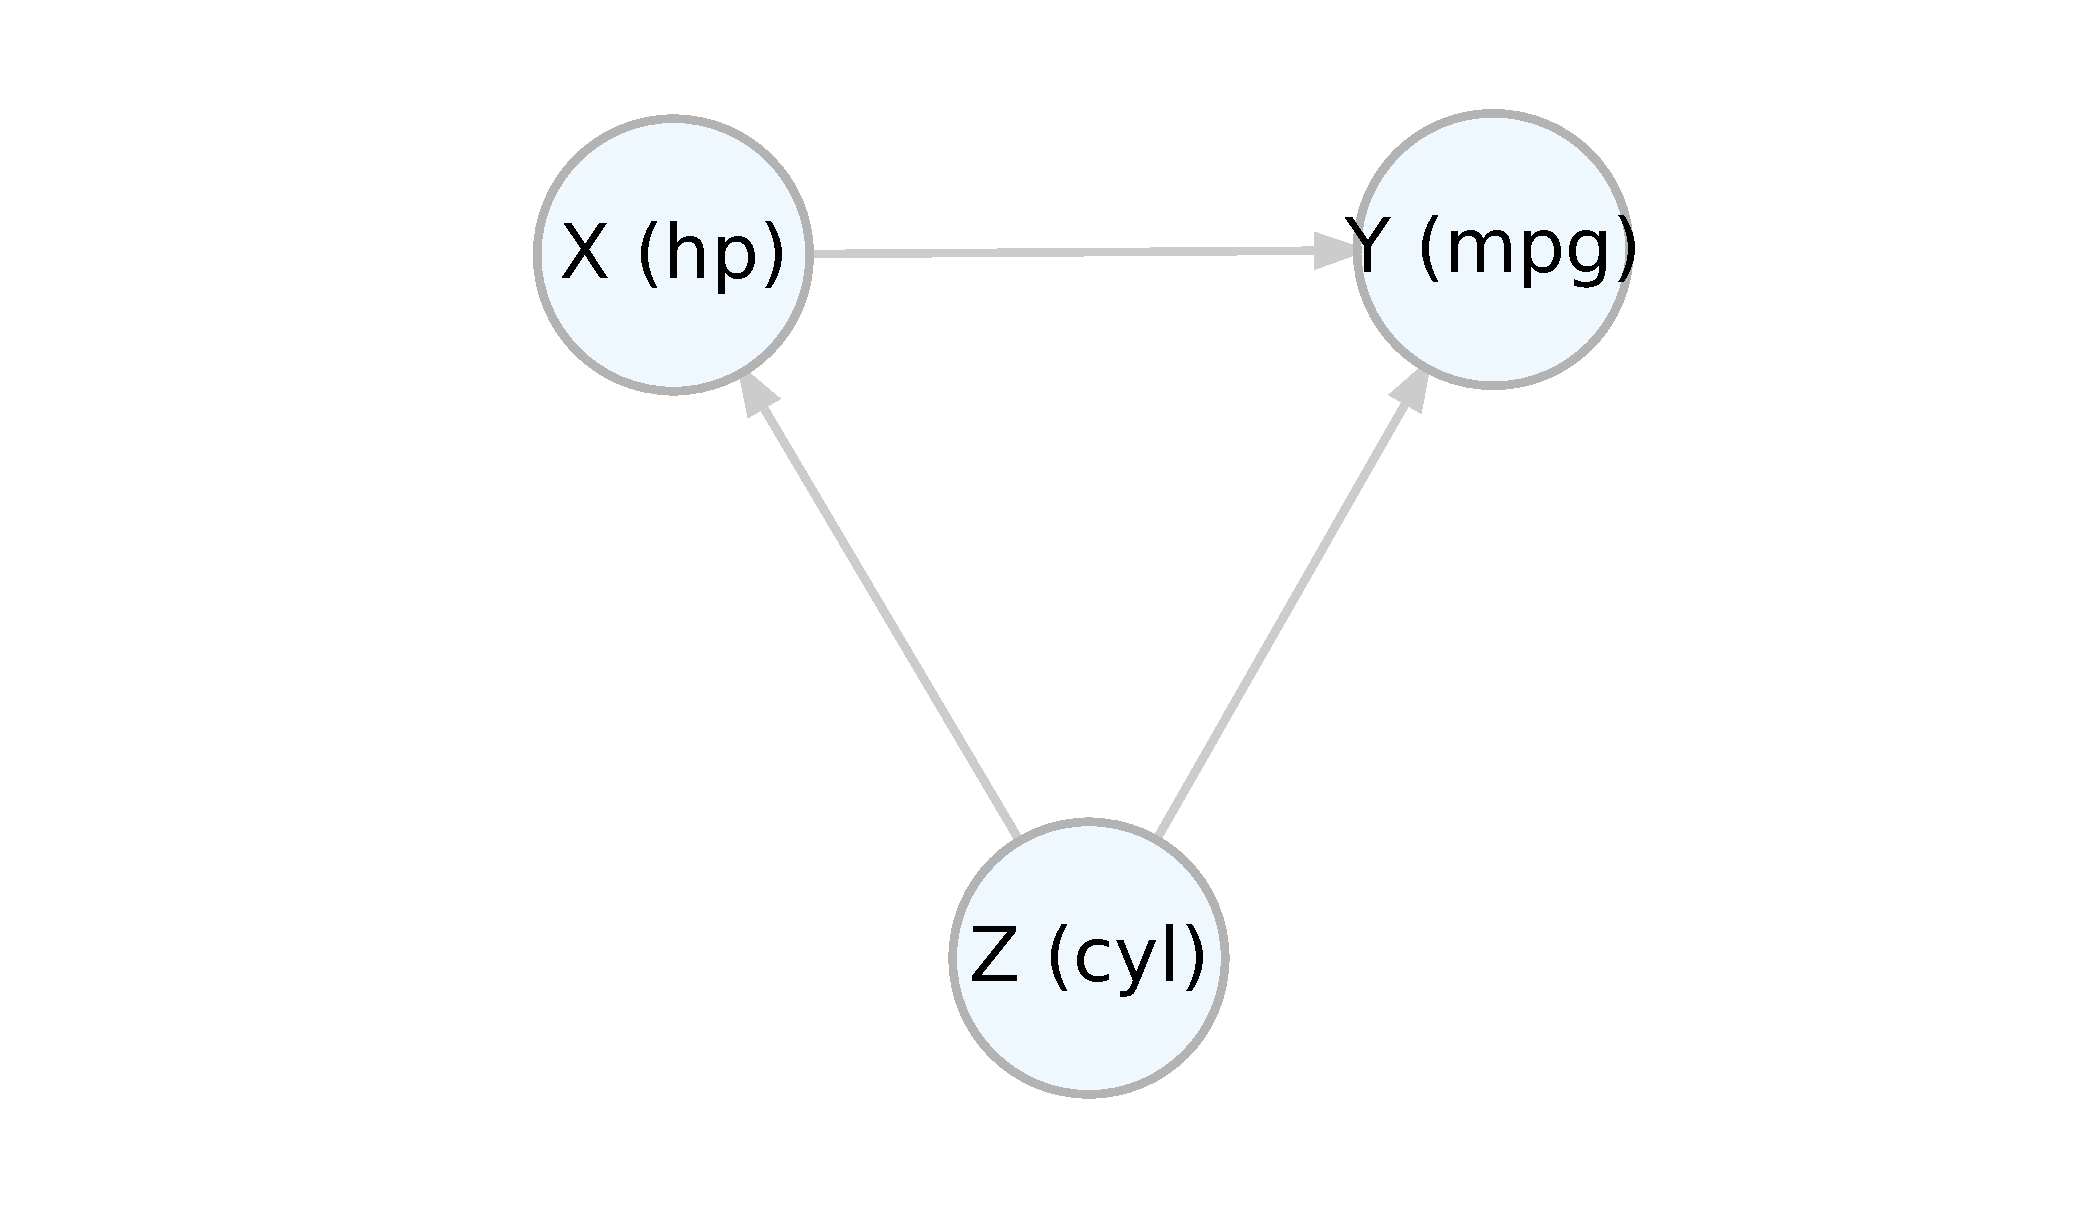
\includegraphics[width=0.35\linewidth,height=0.35\textheight]{_main_files/figure-latex/unnamed-chunk-31-1}

\begin{center}\rule{0.5\linewidth}{0.5pt}\end{center}

\hypertarget{take-a-look-at-the-structure-of-the-mtcars-data-set}{%
\subsection{Take a look at the structure of the mtcars data set}\label{take-a-look-at-the-structure-of-the-mtcars-data-set}}

\begin{verbatim}
## 'data.frame':    32 obs. of  11 variables:
##  $ mpg : num  21 21 22.8 21.4 18.7 18.1 14.3 24.4 22.8 19.2 ...
##  $ cyl : num  6 6 4 6 8 6 8 4 4 6 ...
##  $ disp: num  160 160 108 258 360 ...
##  $ hp  : num  110 110 93 110 175 105 245 62 95 123 ...
##  $ drat: num  3.9 3.9 3.85 3.08 3.15 2.76 3.21 3.69 3.92 3.92 ...
##  $ wt  : num  2.62 2.88 2.32 3.21 3.44 ...
##  $ qsec: num  16.5 17 18.6 19.4 17 ...
##  $ vs  : num  0 0 1 1 0 1 0 1 1 1 ...
##  $ am  : num  1 1 1 0 0 0 0 0 0 0 ...
##  $ gear: num  4 4 4 3 3 3 3 4 4 4 ...
##  $ carb: num  4 4 1 1 2 1 4 2 2 4 ...
\end{verbatim}

\hypertarget{description-of-the-variables-in-the-mtcars-data-set}{%
\subsection{Description of the variables in the mtcars data set}\label{description-of-the-variables-in-the-mtcars-data-set}}

A data frame with 32 observations on 11 (numeric) variables.

\begin{itemize}
\tightlist
\item
  Column 1 = mpg - Miles/(US) gallon
\item
  Column 2 = cyl - Number of cylinders
\item
  Column 3 = disp - Displacement (cu.in.)
\item
  Column 4 = hp - Gross horsepower
\item
  Column 5 = drat - Rear axle ratio
\item
  Column 6 = wt - Weight (1000 lbs)
\item
  Column 7 = qsec - 1/4 mile time
\item
  Column 8 = vs - Engine (0 = V-shaped, 1 = straight)
\item
  Column 9 = am - Transmission (0 = automatic, 1 = manual)
\item
  Column 10 = gear - Number of forward gears
\item
  Column 11 = carb - Number of carburetors
\end{itemize}

\hypertarget{correlation-between-predictor-and-criterion-or-x-and-y}{%
\subsubsection{Correlation between Predictor and Criterion or X and Y}\label{correlation-between-predictor-and-criterion-or-x-and-y}}

Here we find the correlation between our mpg and hp

\begin{Shaded}
\begin{Highlighting}[]
\FunctionTok{cor.test}\NormalTok{(mtcars}\SpecialCharTok{$}\NormalTok{mpg,mtcars}\SpecialCharTok{$}\NormalTok{hp)}
\end{Highlighting}
\end{Shaded}

\begin{verbatim}
## 
##  Pearson's product-moment correlation
## 
## data:  mtcars$mpg and mtcars$hp
## t = -6.7424, df = 30, p-value = 1.788e-07
## alternative hypothesis: true correlation is not equal to 0
## 95 percent confidence interval:
##  -0.8852686 -0.5860994
## sample estimates:
##        cor 
## -0.7761684
\end{verbatim}

\hypertarget{correlation-between-predictor-and-control-or-x-and-z}{%
\subsubsection{Correlation between Predictor and Control or X and Z}\label{correlation-between-predictor-and-control-or-x-and-z}}

Here we find the correlation between our hp and cyl

\begin{Shaded}
\begin{Highlighting}[]
\FunctionTok{cor.test}\NormalTok{(mtcars}\SpecialCharTok{$}\NormalTok{hp,mtcars}\SpecialCharTok{$}\NormalTok{cyl)}
\end{Highlighting}
\end{Shaded}

\begin{verbatim}
## 
##  Pearson's product-moment correlation
## 
## data:  mtcars$hp and mtcars$cyl
## t = 8.2286, df = 30, p-value = 3.478e-09
## alternative hypothesis: true correlation is not equal to 0
## 95 percent confidence interval:
##  0.6816016 0.9154223
## sample estimates:
##       cor 
## 0.8324475
\end{verbatim}

\hypertarget{correlation-between-criterion-and-control-or-y-and-z}{%
\subsubsection{Correlation between Criterion and Control or Y and Z}\label{correlation-between-criterion-and-control-or-y-and-z}}

Here we find the correlation between our mpg and cyl

\begin{Shaded}
\begin{Highlighting}[]
\FunctionTok{cor.test}\NormalTok{(mtcars}\SpecialCharTok{$}\NormalTok{mpg,mtcars}\SpecialCharTok{$}\NormalTok{cyl)}
\end{Highlighting}
\end{Shaded}

\begin{verbatim}
## 
##  Pearson's product-moment correlation
## 
## data:  mtcars$mpg and mtcars$cyl
## t = -8.9197, df = 30, p-value = 6.113e-10
## alternative hypothesis: true correlation is not equal to 0
## 95 percent confidence interval:
##  -0.9257694 -0.7163171
## sample estimates:
##       cor 
## -0.852162
\end{verbatim}

\hypertarget{partial-correlation-putting-it-altogether}{%
\subsection{Partial Correlation: Putting it altogether}\label{partial-correlation-putting-it-altogether}}

\begin{Shaded}
\begin{Highlighting}[]
\DocumentationTok{\#\#\#Partial Correlation when controlling for another variable}
\DocumentationTok{\#\#\#X is hp}
\DocumentationTok{\#\#\#Y is mpg}
\DocumentationTok{\#\#\#Z is cyl}
\NormalTok{xy }\OtherTok{\textless{}{-}} \FunctionTok{cor}\NormalTok{(mtcars}\SpecialCharTok{$}\NormalTok{mpg,mtcars}\SpecialCharTok{$}\NormalTok{hp)}
\NormalTok{xz }\OtherTok{\textless{}{-}} \FunctionTok{cor}\NormalTok{(mtcars}\SpecialCharTok{$}\NormalTok{hp,mtcars}\SpecialCharTok{$}\NormalTok{cyl)}
\NormalTok{yz }\OtherTok{\textless{}{-}} \FunctionTok{cor}\NormalTok{(mtcars}\SpecialCharTok{$}\NormalTok{mpg,mtcars}\SpecialCharTok{$}\NormalTok{cyl)}

\FunctionTok{print}\NormalTok{(xy)}
\end{Highlighting}
\end{Shaded}

\begin{verbatim}
## [1] -0.7761684
\end{verbatim}

\begin{Shaded}
\begin{Highlighting}[]
\FunctionTok{print}\NormalTok{(xz)}
\end{Highlighting}
\end{Shaded}

\begin{verbatim}
## [1] 0.8324475
\end{verbatim}

\begin{Shaded}
\begin{Highlighting}[]
\FunctionTok{print}\NormalTok{(yz)}
\end{Highlighting}
\end{Shaded}

\begin{verbatim}
## [1] -0.852162
\end{verbatim}

\hypertarget{calculate-the-numerator-of-the-formula}{%
\subsection{Calculate the numerator of the formula}\label{calculate-the-numerator-of-the-formula}}

\[\large
r_{xy} - r_{xz}  \cdot r_{yz}
\]

\[\large
-0.7761684 - (0.8324475  \cdot -0.852162)
\]

\begin{Shaded}
\begin{Highlighting}[]
\DocumentationTok{\#\#\#Top of the Formula}
\NormalTok{top\_of\_formula}\OtherTok{\textless{}{-}}\NormalTok{ xy }\SpecialCharTok{{-}}\NormalTok{ (xz}\SpecialCharTok{*}\NormalTok{yz)}
\FunctionTok{print}\NormalTok{(top\_of\_formula)}
\end{Highlighting}
\end{Shaded}

\begin{verbatim}
## [1] -0.06678832
\end{verbatim}

\hypertarget{calculate-the-denominator-of-the-formula}{%
\subsection{Calculate the denominator of the formula}\label{calculate-the-denominator-of-the-formula}}

\[\large
\sqrt{(1-r_{xz}^2) \cdot (1 - r_{yz}^2)}
\]

\[\large
\sqrt{(1-0.8324475^2) \cdot (1 - (-0.852162)^2)}
\]

\begin{Shaded}
\begin{Highlighting}[]
\DocumentationTok{\#\#\#Bottom of formula}
\NormalTok{bottom\_of\_formula}\OtherTok{\textless{}{-}} \FunctionTok{sqrt}\NormalTok{((}\DecValTok{1}\SpecialCharTok{{-}}\NormalTok{(xz}\SpecialCharTok{\^{}}\DecValTok{2}\NormalTok{))}\SpecialCharTok{*}\NormalTok{(}\DecValTok{1}\SpecialCharTok{{-}}\NormalTok{(yz}\SpecialCharTok{\^{}}\DecValTok{2}\NormalTok{)))}
\FunctionTok{print}\NormalTok{(bottom\_of\_formula)}
\end{Highlighting}
\end{Shaded}

\begin{verbatim}
## [1] 0.2899505
\end{verbatim}

\begin{Shaded}
\begin{Highlighting}[]
\NormalTok{final\_answer}\OtherTok{=}\NormalTok{ top\_of\_formula}\SpecialCharTok{/}\NormalTok{bottom\_of\_formula}
\FunctionTok{print}\NormalTok{(final\_answer)}
\end{Highlighting}
\end{Shaded}

\begin{verbatim}
## [1] -0.2303439
\end{verbatim}

\begin{Shaded}
\begin{Highlighting}[]
\FunctionTok{print}\NormalTok{(}\FunctionTok{round}\NormalTok{(final\_answer,}\DecValTok{2}\NormalTok{))}
\end{Highlighting}
\end{Shaded}

\begin{verbatim}
## [1] -0.23
\end{verbatim}

Note: Round up at the very end of the calculation.

\[\large
r = \frac{-0.06678832}{0.2899505}
\]
\[\large
r = -0.230439
\]

\hypertarget{partial-correlation-utilizing-the-ppcor-package}{%
\subsection{Partial Correlation utilizing the ppcor package}\label{partial-correlation-utilizing-the-ppcor-package}}

\textbf{First order partial coefficient} -- is a correlation between two variables with just one additional variable partialed out of both.

Here we can utilize the ppcor package as an easy button method to calculate the partial correlation. You will need to install the ppcor package via CRAN: \href{https://cran.r-project.org/web/packages/ppcor/index.html}{ppcor package}

\begin{Shaded}
\begin{Highlighting}[]
\DocumentationTok{\#\#\#Partial Correlation when controlling for another variable}
\DocumentationTok{\#\#Load the ppcor library}
\FunctionTok{library}\NormalTok{(ppcor)}
\end{Highlighting}
\end{Shaded}

\begin{verbatim}
## Loading required package: MASS
\end{verbatim}

\begin{verbatim}
## 
## Attaching package: 'MASS'
\end{verbatim}

\begin{verbatim}
## The following object is masked from 'package:dplyr':
## 
##     select
\end{verbatim}

\begin{Shaded}
\begin{Highlighting}[]
\DocumentationTok{\#\#\#ppcor function controlling for cylinders in the mtcars dataset}
\NormalTok{ppcor}\SpecialCharTok{::}\FunctionTok{pcor.test}\NormalTok{(mtcars}\SpecialCharTok{$}\NormalTok{mpg, mtcars}\SpecialCharTok{$}\NormalTok{hp, mtcars[, }\FunctionTok{c}\NormalTok{(}\StringTok{"cyl"}\NormalTok{)])}
\end{Highlighting}
\end{Shaded}

\begin{verbatim}
##     estimate   p.value statistic  n gp  Method
## 1 -0.2303439 0.2125285 -1.274718 32  1 pearson
\end{verbatim}

\hypertarget{higher-order-partial-correlation-is-a-correlation-between-two-variables-with-more-than-one-control-variable-partialed-out-by-both.}{%
\subsubsection{Higher order partial correlation -- is a correlation between two variables with more than one control variable partialed out by both.}\label{higher-order-partial-correlation-is-a-correlation-between-two-variables-with-more-than-one-control-variable-partialed-out-by-both.}}

\begin{Shaded}
\begin{Highlighting}[]
\DocumentationTok{\#\#\#ppcor function controlling for cylinders,displacement in the mtcars dataset}
\NormalTok{ppcor}\SpecialCharTok{::}\FunctionTok{pcor.test}\NormalTok{(mtcars}\SpecialCharTok{$}\NormalTok{mpg, mtcars}\SpecialCharTok{$}\NormalTok{hp, mtcars[, }\FunctionTok{c}\NormalTok{(}\StringTok{"cyl"}\NormalTok{,}\StringTok{"disp"}\NormalTok{)])}
\end{Highlighting}
\end{Shaded}

\begin{verbatim}
##     estimate   p.value statistic  n gp  Method
## 1 -0.1860437 0.3249519 -1.001943 32  2 pearson
\end{verbatim}

\hypertarget{references}{%
\subsubsection{References}\label{references}}

Hatcher, L. (2013). \emph{Advanced statistics in research: Reading, understanding, and writing up data analysis results. Shadow Finch Media.}

Henderson and Velleman (1981), \emph{Building multiple regression models interactively.} Biometrics, 37, 391--411.

Kim S (2015). \emph{ppcor: Partial and Semi-Partial (Part) Correlation}. R package version 1.1, \url{https://CRAN.R-project.org/package=ppcor}.

\hypertarget{bivariate-regression-terminology}{%
\subsection{Bivariate Regression Terminology}\label{bivariate-regression-terminology}}

\begin{itemize}
\item
  \textbf{Regression} -- is the process of estimating a best-fitting line that summarizes the relationship between a predictor variable (Independent Variable) and a criterion variable (Dependent Variable).
\item
  \textbf{Regression Analysis} -- researchers fit a regression line to a sample of data, estimate the parameters of the regression equation (i.e., the constant and regression coefficient), and use the resulting equation to predict scores on a criterion variable.
\item
  \textbf{Bivariate} -- means that the analyses discussed include just 2 variables, a predictor variable (the X variable), and a criterion variable (the Y variable).
\item
  \textbf{Linear} -- refers to the fact, when the Y scores are plotted against the X scores, it should be possible to fit a best-fitting straight line through the center of the scores, as opposed to a best-fitting curved line.
\end{itemize}

\hypertarget{regression-generic-analysis-model}{%
\subsubsection{Regression: Generic Analysis Model}\label{regression-generic-analysis-model}}

\begin{center}\rule{0.5\linewidth}{0.5pt}\end{center}

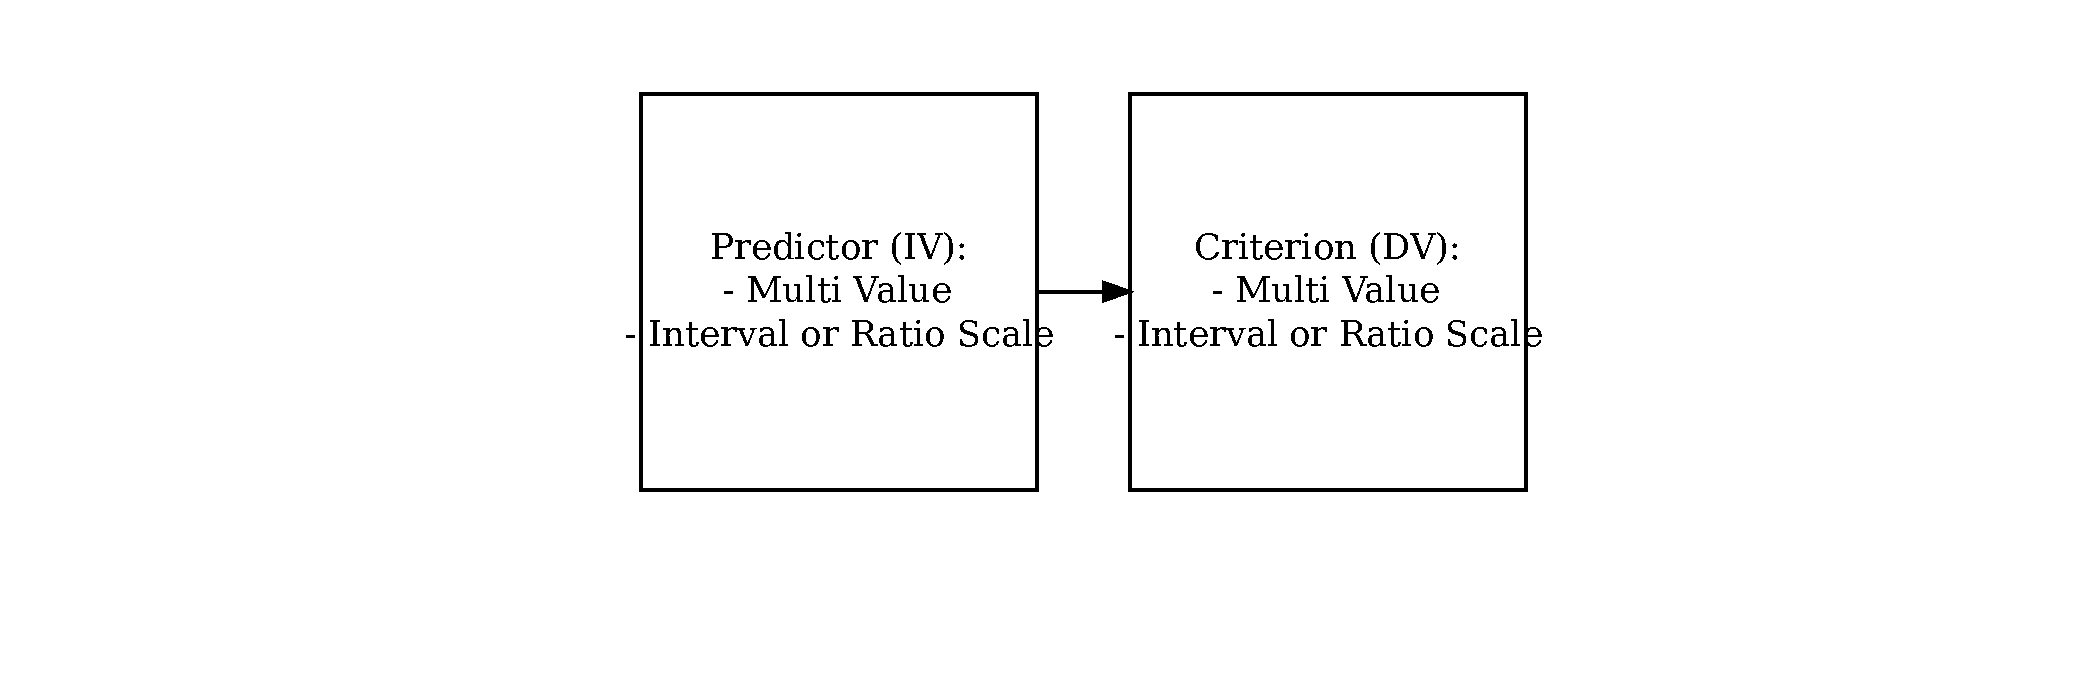
\includegraphics{_main_files/figure-latex/unnamed-chunk-43-1.pdf}

\begin{center}\rule{0.5\linewidth}{0.5pt}\end{center}

\hypertarget{assumptions-of-bivariate-regression}{%
\subsection{Assumptions of Bivariate Regression}\label{assumptions-of-bivariate-regression}}

\begin{itemize}
\item
  \textbf{Linearity} -- should be able to fit a best-fitting straight line through the scatterplot.
\item
  \textbf{Independence} -- each observation included in the sample should be drawn independently from the population of interest. Researchers should not have taken repeated measures on the same variable from the same participant.
\item
  \textbf{Homogeneity of Variance (Homoscedasticity)} -- the variance of the Y scores should remain fairly constant at all values of X.
\item
  \textbf{Normality} -- residuals of prediction should be normally distributed.
  Bivariate Normality -- for any specific score on one of the variables, scores on the other variable should follow a normal distribution.
\end{itemize}

\hypertarget{bivariate-regression-formula}{%
\subsection{Bivariate Regression Formula}\label{bivariate-regression-formula}}

Here we have the formula for the bivariate regression equation.
The regression equation takes the following form:
\[\Large
Regression\;Equation:\;\;\;\hat{y} = a + \beta(X)
\]
\[
\hat{y}\;\;–\;the\;predicted\;score\;on\;the\;criterion\;variable
\]
\[
a\;–\;the\;constant\;or\;the\;intercept\;of\;the\;regression\;equation.
\]
\[
\beta\;–\;the\;unstandardized\;regression\;coefficient.\\Represents\;the\;amount\;of\;change\;in\;Y\;that\;is \;associated\;with\;a\;one-unit\;change\;in\;X\;\\when\;both\;variables\;are\;in\;raw\;score\;form.\;Also\;known\;as\;the\;regression\;weight\;or\;slope.
\]

\hypertarget{scatterplot-of-the-data-set}{%
\subsection{Scatterplot of the data set}\label{scatterplot-of-the-data-set}}

Here we plot our data to get a good look at the shape of the data set.

\begin{itemize}
\tightlist
\item
  \textbf{Scatterplot} -- a graph that illustrates the nature of the relationship between two quantitative variables.
\item
  \textbf{X Axis} -- Predictor Variable - hp
\item
  \textbf{Y Axis} -- Criterion Variable - mpg
\end{itemize}

We can utilize the following plot function to create a basic scatterplot in R.

\begin{Shaded}
\begin{Highlighting}[]
\FunctionTok{attach}\NormalTok{(mtcars)}
\FunctionTok{with}\NormalTok{(}\AttributeTok{data =}\NormalTok{ mtcars,}\FunctionTok{plot}\NormalTok{(}\AttributeTok{x =}\NormalTok{ hp,}\AttributeTok{y =}\NormalTok{ mpg,}\AttributeTok{col=}\StringTok{"black"}\NormalTok{,}\AttributeTok{pch=}\DecValTok{19}\NormalTok{,}\AttributeTok{main=}\StringTok{"Mtcars"}\NormalTok{))}
\end{Highlighting}
\end{Shaded}

\begin{verbatim}
## The following object is masked from package:ggplot2:
## 
##     mpg
\end{verbatim}

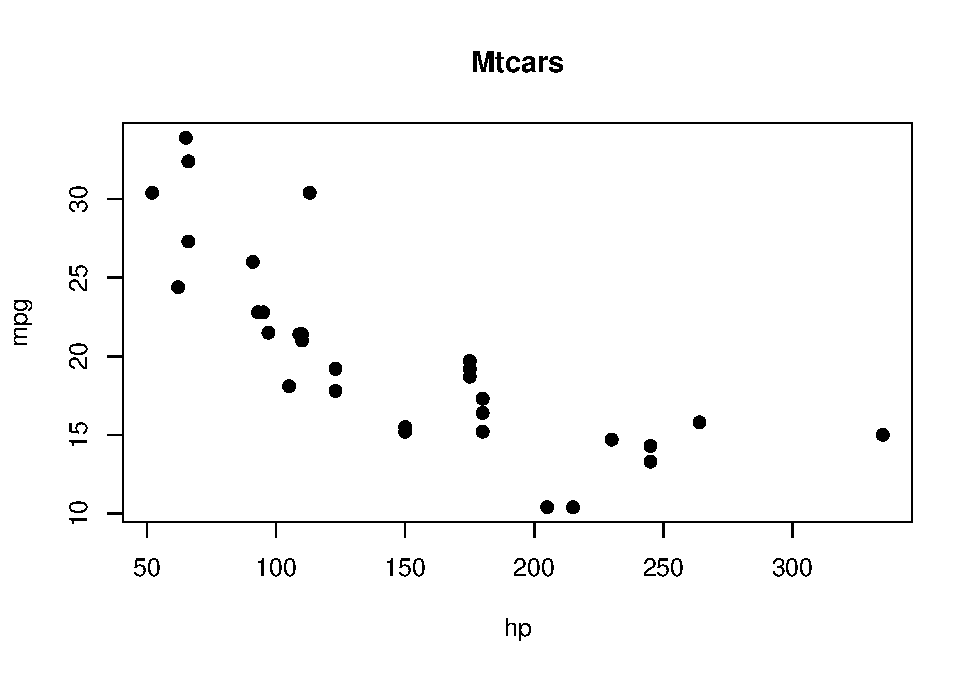
\includegraphics{_main_files/figure-latex/unnamed-chunk-45-1.pdf}

\hypertarget{calculate-the-residual}{%
\subsection{Calculate the Residual}\label{calculate-the-residual}}

Here we compute the residual by taking the actual y value and subtract the predicted y value. The residual for each observation is the difference between the predicted values of y and the actual values of y. Calculating the residual helps us to see if we have overpredicted or underpredicted for \(\hat{y}\).

\[\Large
Residual = actual\;y\;value - predicted\;y\;value
\]

\[\Large
r_{1} = y_{i} - \hat{y_{i}}
\]

\begin{verbatim}
## [1] "Predicted y Values"
\end{verbatim}

\begin{verbatim}
##           Mazda RX4       Mazda RX4 Wag          Datsun 710      Hornet 4 Drive 
##           22.593750           22.593750           23.753631           22.593750 
##   Hornet Sportabout             Valiant          Duster 360           Merc 240D 
##           18.158912           22.934891           13.382932           25.868707 
##            Merc 230            Merc 280           Merc 280C          Merc 450SE 
##           23.617174           21.706782           21.706782           17.817770 
##          Merc 450SL         Merc 450SLC  Cadillac Fleetwood Lincoln Continental 
##           17.817770           17.817770           16.112064           15.429781 
##   Chrysler Imperial            Fiat 128         Honda Civic      Toyota Corolla 
##           14.406357           25.595794           26.550990           25.664022 
##       Toyota Corona    Dodge Challenger         AMC Javelin          Camaro Z28 
##           23.480718           19.864619           19.864619           13.382932 
##    Pontiac Firebird           Fiat X1-9       Porsche 914-2        Lotus Europa 
##           18.158912           25.595794           23.890087           22.389065 
##      Ford Pantera L        Ferrari Dino       Maserati Bora          Volvo 142E 
##           12.086595           18.158912            7.242387           22.661978
\end{verbatim}

\begin{verbatim}
## [1] "Actual y Values"
\end{verbatim}

\begin{verbatim}
##  [1] 21.0 21.0 22.8 21.4 18.7 18.1 14.3 24.4 22.8 19.2 17.8 16.4 17.3 15.2 10.4
## [16] 10.4 14.7 32.4 30.4 33.9 21.5 15.5 15.2 13.3 19.2 27.3 26.0 30.4 15.8 19.7
## [31] 15.0 21.4
\end{verbatim}

\begin{verbatim}
## [1] "Manually Calculated Residuals"
\end{verbatim}

\begin{verbatim}
##                     mtcars$mpg - mpg_prediction$fitted.values
## Mazda RX4                                         -1.59374995
## Mazda RX4 Wag                                     -1.59374995
## Datsun 710                                        -0.95363068
## Hornet 4 Drive                                    -1.19374995
## Hornet Sportabout                                  0.54108812
## Valiant                                           -4.83489134
## Duster 360                                         0.91706759
## Merc 240D                                         -1.46870730
## Merc 230                                          -0.81717412
## Merc 280                                          -2.50678234
## Merc 280C                                         -3.90678234
## Merc 450SE                                        -1.41777049
## Merc 450SL                                        -0.51777049
## Merc 450SLC                                       -2.61777049
## Cadillac Fleetwood                                -5.71206353
## Lincoln Continental                               -5.02978075
## Chrysler Imperial                                  0.29364342
## Fiat 128                                           6.80420581
## Honda Civic                                        3.84900992
## Toyota Corolla                                     8.23597754
## Toyota Corona                                     -1.98071757
## Dodge Challenger                                  -4.36461883
## AMC Javelin                                       -4.66461883
## Camaro Z28                                        -0.08293241
## Pontiac Firebird                                   1.04108812
## Fiat X1-9                                          1.70420581
## Porsche 914-2                                      2.10991276
## Lotus Europa                                       8.01093488
## Ford Pantera L                                     3.71340487
## Ferrari Dino                                       1.54108812
## Maserati Bora                                      7.75761261
## Volvo 142E                                        -1.26197823
\end{verbatim}

\begin{verbatim}
## [1] "Residual Values"
\end{verbatim}

\begin{verbatim}
##           Mazda RX4       Mazda RX4 Wag          Datsun 710      Hornet 4 Drive 
##         -1.59374995         -1.59374995         -0.95363068         -1.19374995 
##   Hornet Sportabout             Valiant          Duster 360           Merc 240D 
##          0.54108812         -4.83489134          0.91706759         -1.46870730 
##            Merc 230            Merc 280           Merc 280C          Merc 450SE 
##         -0.81717412         -2.50678234         -3.90678234         -1.41777049 
##          Merc 450SL         Merc 450SLC  Cadillac Fleetwood Lincoln Continental 
##         -0.51777049         -2.61777049         -5.71206353         -5.02978075 
##   Chrysler Imperial            Fiat 128         Honda Civic      Toyota Corolla 
##          0.29364342          6.80420581          3.84900992          8.23597754 
##       Toyota Corona    Dodge Challenger         AMC Javelin          Camaro Z28 
##         -1.98071757         -4.36461883         -4.66461883         -0.08293241 
##    Pontiac Firebird           Fiat X1-9       Porsche 914-2        Lotus Europa 
##          1.04108812          1.70420581          2.10991276          8.01093488 
##      Ford Pantera L        Ferrari Dino       Maserati Bora          Volvo 142E 
##          3.71340487          1.54108812          7.75761261         -1.26197823
\end{verbatim}

\hypertarget{calculate-the-mean-of-the-y-values}{%
\subsection{Calculate the mean of the Y Values}\label{calculate-the-mean-of-the-y-values}}

Here we find the mean of our criterion (y) value of mpg.

\[\Large
\bar{y} = \frac{\sum{y}}{n}
\]

We can utilize the \textbf{\emph{mean}} function to the calculate the mean of mpg (miles per gallon).

\begin{Shaded}
\begin{Highlighting}[]
\FunctionTok{mean}\NormalTok{(mtcars}\SpecialCharTok{$}\NormalTok{mpg)}
\end{Highlighting}
\end{Shaded}

\begin{verbatim}
## [1] 20.09062
\end{verbatim}

\hypertarget{coefficient-of-determination-or-r2}{%
\subsection{\texorpdfstring{Coefficient of Determination or \({R^2}\)}{Coefficient of Determination or \{R\^{}2\}}}\label{coefficient-of-determination-or-r2}}

\textbf{Coefficient of Determination} -- indicates the percent of \textbf{variance in the criterion} variable \textbf{that is accounted for by the predictor} variable.

\begin{center}\rule{0.5\linewidth}{0.5pt}\end{center}

\[
Coefficient\;of\;Determination:\;\;R^2 =\;1-\; \frac{sum\;squared\;regression\;(SSR)}{sum\;squares\;total\;(SST)}
\]

\[
=1- \frac{\sum(y_{i}\;-\;\hat{y_{i}})^2}{\sum(y_{i}\;-\;\overline{y})^2}
\\
\\
y_{i} = actual\;y\;values
\\
\hat{y_i} = predicted\;y\;values
\\
\overline{y} = mean\;of\;y
\\
\sum\;or\;sigma = sum
\]

\begin{center}\rule{0.5\linewidth}{0.5pt}\end{center}

\hypertarget{calculate-the-numerator-of-the-formula---sum-squared-regression-ssr}{%
\subsection{Calculate the numerator of the formula - Sum Squared Regression (SSR)}\label{calculate-the-numerator-of-the-formula---sum-squared-regression-ssr}}

\[
\sum(y_{i}\;-\;\hat{y_{i}})^2
\]

\begin{Shaded}
\begin{Highlighting}[]
\NormalTok{top\_of\_formula }\OtherTok{\textless{}{-}} \FunctionTok{sum}\NormalTok{(mpg\_prediction}\SpecialCharTok{$}\NormalTok{residuals}\SpecialCharTok{\^{}}\DecValTok{2}\NormalTok{)}
\FunctionTok{print}\NormalTok{(top\_of\_formula)}
\end{Highlighting}
\end{Shaded}

\begin{verbatim}
## [1] 447.6743
\end{verbatim}

\hypertarget{calculate-the-denominator-of-the-formula---sum-squares-total-sst}{%
\subsection{Calculate the denominator of the formula - Sum Squares Total (SST)}\label{calculate-the-denominator-of-the-formula---sum-squares-total-sst}}

\begin{center}\rule{0.5\linewidth}{0.5pt}\end{center}

\[
\sum(y_{i}\;-\;\overline{y})^2
\]

\begin{center}\rule{0.5\linewidth}{0.5pt}\end{center}

\begin{Shaded}
\begin{Highlighting}[]
\NormalTok{bottom\_of\_formula }\OtherTok{\textless{}{-}} \FunctionTok{sum}\NormalTok{((mtcars}\SpecialCharTok{$}\NormalTok{mpg}\SpecialCharTok{{-}}\FunctionTok{mean}\NormalTok{(mtcars}\SpecialCharTok{$}\NormalTok{mpg))}\SpecialCharTok{\^{}}\DecValTok{2}\NormalTok{)}
\FunctionTok{print}\NormalTok{(bottom\_of\_formula)}
\end{Highlighting}
\end{Shaded}

\begin{verbatim}
## [1] 1126.047
\end{verbatim}

\begin{center}\rule{0.5\linewidth}{0.5pt}\end{center}

\[
R^2 = 1- \frac{447.6743}{1126.047}
\]
\[
R^2 = 1- 0.3975627
\]
\[
R^2 = 0.6024373
\\
R^2 = 0.6024
\]

\begin{center}\rule{0.5\linewidth}{0.5pt}\end{center}

\hypertarget{calculate-the-adjusted-r-squared-adj.r2orr2_adj}{%
\subsection{\texorpdfstring{Calculate the Adjusted-R Squared \(Adj.R^2\;or\;R^2_{adj}\)}{Calculate the Adjusted-R Squared Adj.R\^{}2\textbackslash;or\textbackslash;R\^{}2\_\{adj\}}}\label{calculate-the-adjusted-r-squared-adj.r2orr2_adj}}

\begin{center}\rule{0.5\linewidth}{0.5pt}\end{center}

\[
Adj.R^2\;or\;R^2_{adj} = 1 - (1-R^2)\;\cdot\;(n-1)/(n-p-1)
\\
Adj.R^2\;or\;R^2_{adj} = 1 - (1-0.6024373)\;\cdot\;(32-1)/(32-1-1)
\\
R^2 = coefficient\;of\;determination
\\
n = number\;of\;observations
\\
p=number\;of\;predictors
\]

\begin{center}\rule{0.5\linewidth}{0.5pt}\end{center}

\begin{center}\rule{0.5\linewidth}{0.5pt}\end{center}

\begin{Shaded}
\begin{Highlighting}[]
\NormalTok{adj.r.squared }\OtherTok{=} \DecValTok{1} \SpecialCharTok{{-}}\NormalTok{ (}\DecValTok{1} \SpecialCharTok{{-}} \FloatTok{0.6024373}\NormalTok{) }\SpecialCharTok{*}\NormalTok{ ((}\DecValTok{32} \SpecialCharTok{{-}} \DecValTok{1}\NormalTok{)}\SpecialCharTok{/}\NormalTok{(}\DecValTok{32{-}1{-}1}\NormalTok{))}
\FunctionTok{print}\NormalTok{(adj.r.squared)}
\end{Highlighting}
\end{Shaded}

\begin{verbatim}
## [1] 0.5891852
\end{verbatim}

\hypertarget{utilize-the-lm-function-in-r-to-automate-our-work}{%
\subsection{Utilize the lm function in R to automate our work}\label{utilize-the-lm-function-in-r-to-automate-our-work}}

Here we can utilize the \textbf{\emph{lm}} function in R to perform our bivariate regression (simple linear regression). This will allow us to save the model to a variable and then utilize the \textbf{\$} (dollar sign) operator in R. The \textbf{\$} (dollar sign) operator allows us to pull out things we need such as the residuals and fitted values that are returned from the summary function.

\hypertarget{print-the-residuals-of-the-model}{%
\subsubsection{Print the residuals of the model}\label{print-the-residuals-of-the-model}}

\begin{Shaded}
\begin{Highlighting}[]
\NormalTok{mpg\_hp\_model }\OtherTok{\textless{}{-}} \FunctionTok{lm}\NormalTok{(mpg }\SpecialCharTok{\textasciitilde{}}\NormalTok{ hp, mtcars)}
\FunctionTok{print}\NormalTok{(mpg\_hp\_model}\SpecialCharTok{$}\NormalTok{residuals)}
\end{Highlighting}
\end{Shaded}

\begin{verbatim}
##           Mazda RX4       Mazda RX4 Wag          Datsun 710      Hornet 4 Drive 
##         -1.59374995         -1.59374995         -0.95363068         -1.19374995 
##   Hornet Sportabout             Valiant          Duster 360           Merc 240D 
##          0.54108812         -4.83489134          0.91706759         -1.46870730 
##            Merc 230            Merc 280           Merc 280C          Merc 450SE 
##         -0.81717412         -2.50678234         -3.90678234         -1.41777049 
##          Merc 450SL         Merc 450SLC  Cadillac Fleetwood Lincoln Continental 
##         -0.51777049         -2.61777049         -5.71206353         -5.02978075 
##   Chrysler Imperial            Fiat 128         Honda Civic      Toyota Corolla 
##          0.29364342          6.80420581          3.84900992          8.23597754 
##       Toyota Corona    Dodge Challenger         AMC Javelin          Camaro Z28 
##         -1.98071757         -4.36461883         -4.66461883         -0.08293241 
##    Pontiac Firebird           Fiat X1-9       Porsche 914-2        Lotus Europa 
##          1.04108812          1.70420581          2.10991276          8.01093488 
##      Ford Pantera L        Ferrari Dino       Maserati Bora          Volvo 142E 
##          3.71340487          1.54108812          7.75761261         -1.26197823
\end{verbatim}

\hypertarget{print-the-coefficients-of-the-model}{%
\subsubsection{Print the coefficients of the model}\label{print-the-coefficients-of-the-model}}

\begin{Shaded}
\begin{Highlighting}[]
\NormalTok{mpg\_hp\_model }\OtherTok{\textless{}{-}} \FunctionTok{lm}\NormalTok{(mpg }\SpecialCharTok{\textasciitilde{}}\NormalTok{ hp, mtcars)}
\FunctionTok{print}\NormalTok{(mpg\_hp\_model}\SpecialCharTok{$}\NormalTok{coefficients)}
\end{Highlighting}
\end{Shaded}

\begin{verbatim}
## (Intercept)          hp 
## 30.09886054 -0.06822828
\end{verbatim}

\hypertarget{print-the-fitted-values-of-the-model}{%
\subsubsection{Print the fitted values of the model}\label{print-the-fitted-values-of-the-model}}

\begin{Shaded}
\begin{Highlighting}[]
\NormalTok{mpg\_hp\_model }\OtherTok{\textless{}{-}} \FunctionTok{lm}\NormalTok{(mpg }\SpecialCharTok{\textasciitilde{}}\NormalTok{ hp, mtcars)}
\FunctionTok{print}\NormalTok{(mpg\_hp\_model}\SpecialCharTok{$}\NormalTok{fitted.values)}
\end{Highlighting}
\end{Shaded}

\begin{verbatim}
##           Mazda RX4       Mazda RX4 Wag          Datsun 710      Hornet 4 Drive 
##           22.593750           22.593750           23.753631           22.593750 
##   Hornet Sportabout             Valiant          Duster 360           Merc 240D 
##           18.158912           22.934891           13.382932           25.868707 
##            Merc 230            Merc 280           Merc 280C          Merc 450SE 
##           23.617174           21.706782           21.706782           17.817770 
##          Merc 450SL         Merc 450SLC  Cadillac Fleetwood Lincoln Continental 
##           17.817770           17.817770           16.112064           15.429781 
##   Chrysler Imperial            Fiat 128         Honda Civic      Toyota Corolla 
##           14.406357           25.595794           26.550990           25.664022 
##       Toyota Corona    Dodge Challenger         AMC Javelin          Camaro Z28 
##           23.480718           19.864619           19.864619           13.382932 
##    Pontiac Firebird           Fiat X1-9       Porsche 914-2        Lotus Europa 
##           18.158912           25.595794           23.890087           22.389065 
##      Ford Pantera L        Ferrari Dino       Maserati Bora          Volvo 142E 
##           12.086595           18.158912            7.242387           22.661978
\end{verbatim}

\hypertarget{putting-it-altogether}{%
\subsubsection{Putting it altogether}\label{putting-it-altogether}}

Here we can print out the summary of the model utilizing the \textbf{\emph{summary}} function in R; \texttt{summary(mpg\_hp\_model)}. We can also plot the predicted y values with the actual y values. Then we can draw a line between each of the predicted values and the actual values.This helps us visualize the amount of variation that is present between the predicted vs the actual values of y.

\begin{Shaded}
\begin{Highlighting}[]
\NormalTok{mpg\_hp\_model }\OtherTok{=} \FunctionTok{lm}\NormalTok{(mpg }\SpecialCharTok{\textasciitilde{}}\NormalTok{ hp, mtcars)}
\FunctionTok{print}\NormalTok{(}\FunctionTok{summary}\NormalTok{(mpg\_hp\_model))}
\end{Highlighting}
\end{Shaded}

\hypertarget{plot-our-residuals-and-a-best-fitting-line}{%
\subsubsection{Plot our residuals and a best fitting line}\label{plot-our-residuals-and-a-best-fitting-line}}

Here we can utilize the \texttt{ggplot2} package to plot our model. We can also plot the residuals along with a best fitting line.

\begin{Shaded}
\begin{Highlighting}[]
\NormalTok{mtcars }\SpecialCharTok{\%\textgreater{}\%} \FunctionTok{ggplot}\NormalTok{(}\FunctionTok{aes}\NormalTok{(hp,mpg))}\SpecialCharTok{+}
  \FunctionTok{geom\_point}\NormalTok{()}\SpecialCharTok{+}
  \FunctionTok{geom\_smooth}\NormalTok{(}\AttributeTok{method =} \StringTok{"lm"}\NormalTok{)}\SpecialCharTok{+}
  \FunctionTok{geom\_linerange}\NormalTok{(}\FunctionTok{aes}\NormalTok{(}\AttributeTok{ymax =}\NormalTok{ mpg, }\AttributeTok{ymin =}\NormalTok{ mpg}\SpecialCharTok{{-}}\NormalTok{resid),}\AttributeTok{color=}\StringTok{"red"}\NormalTok{)}
\end{Highlighting}
\end{Shaded}

\begin{verbatim}
## 
## Call:
## lm(formula = mpg ~ hp, data = mtcars)
## 
## Residuals:
##     Min      1Q  Median      3Q     Max 
## -5.7121 -2.1122 -0.8854  1.5819  8.2360 
## 
## Coefficients:
##             Estimate Std. Error t value Pr(>|t|)    
## (Intercept) 30.09886    1.63392  18.421  < 2e-16 ***
## hp          -0.06823    0.01012  -6.742 1.79e-07 ***
## ---
## Signif. codes:  0 '***' 0.001 '**' 0.01 '*' 0.05 '.' 0.1 ' ' 1
## 
## Residual standard error: 3.863 on 30 degrees of freedom
## Multiple R-squared:  0.6024, Adjusted R-squared:  0.5892 
## F-statistic: 45.46 on 1 and 30 DF,  p-value: 1.788e-07
\end{verbatim}

\begin{verbatim}
## `geom_smooth()` using formula = 'y ~ x'
\end{verbatim}

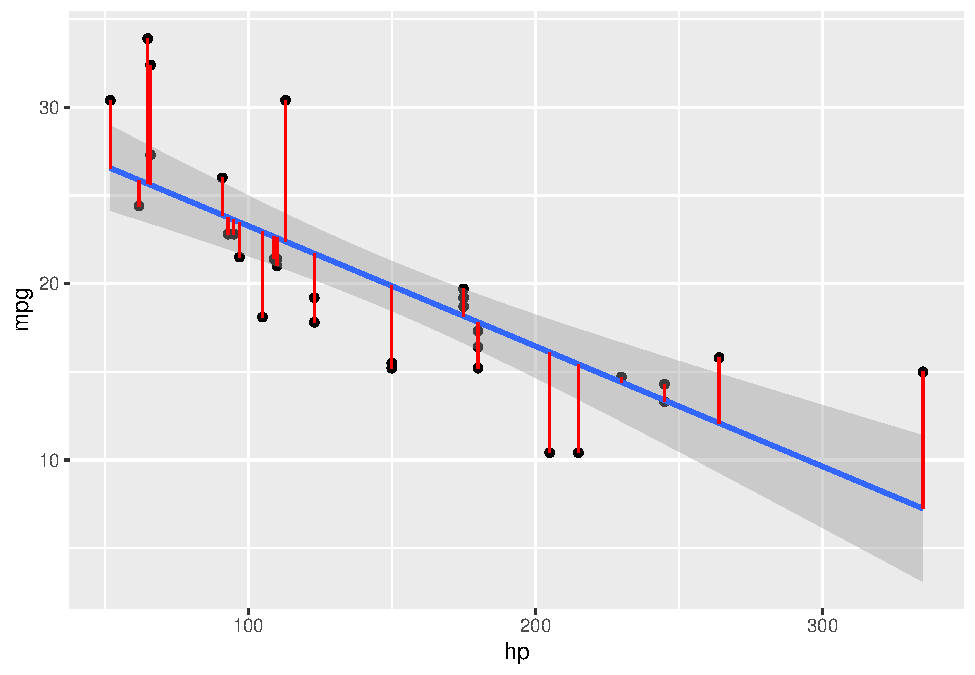
\includegraphics{_main_files/figure-latex/unnamed-chunk-57-1.pdf}

Now we can take a predictor value (X) and plug it in. We then are able to predict where our criterion value (Y) wil be.

\[
\hat{y}\;=\;30.09886\;+\;-0.06823(X)
\]

\[
\hat{y}\;=\;30.09886\;+\;-0.06823(335)
\]
\[
\hat{y}\;=\;30.09886\;+\;-22.85705
\]
\[
\hat{y} = 7.24
\]

\begin{center}\rule{0.5\linewidth}{0.5pt}\end{center}

\hypertarget{squaring-the-correlation-r-to-find-the-coefficient-of-determination-r2}{%
\subsection{\texorpdfstring{Squaring the correlation \({r}\) to find the coefficient of determination \({R^2}\)}{Squaring the correlation \{r\} to find the coefficient of determination \{R\^{}2\}}}\label{squaring-the-correlation-r-to-find-the-coefficient-of-determination-r2}}

According to Hatcher (2013) we can simply square the correlation provided we are looking at only one predictor variable and one dependent variable. When we square the correlation coefficient this will give us the coefficient of determination.

\hypertarget{correlation-coefficient-of-hp-and-mpg}{%
\subsection{Correlation coefficient of hp and mpg}\label{correlation-coefficient-of-hp-and-mpg}}

\begin{Shaded}
\begin{Highlighting}[]
\FunctionTok{cor}\NormalTok{(}\AttributeTok{x =}\NormalTok{ mtcars}\SpecialCharTok{$}\NormalTok{hp,mtcars}\SpecialCharTok{$}\NormalTok{mpg)}
\end{Highlighting}
\end{Shaded}

\begin{verbatim}
## [1] -0.7761684
\end{verbatim}

\({r} = -0.7761684\)

\hypertarget{squaring-the-correlation-coefficient}{%
\subsection{Squaring the correlation coefficient}\label{squaring-the-correlation-coefficient}}

Here we can square the correlation coefficient \({r}\) and it will give us the coefficient of determination or \({R^2}\)

\begin{Shaded}
\begin{Highlighting}[]
\FunctionTok{cor}\NormalTok{(}\AttributeTok{x =}\NormalTok{ mtcars}\SpecialCharTok{$}\NormalTok{hp,mtcars}\SpecialCharTok{$}\NormalTok{mpg)}\SpecialCharTok{\^{}}\DecValTok{2}
\end{Highlighting}
\end{Shaded}

\begin{verbatim}
## [1] 0.6024373
\end{verbatim}

\({R^2} = 0.6024373\)

Here we can see we get the same value for the coefficient of determination \({R^2}\) by squaring the correlation as if we had utilized the \textbf{\emph{lm}} function. However the \textbf{\emph{lm}} function has advantages as it provides us with our p-value, F-statistic, and the intercept and the unstandardized regression coefficient.

\hypertarget{data-set-description}{%
\subsection{Data Set Description}\label{data-set-description}}

Motor Trend Car Road Tests

Description:

The data was extracted from the 1974 Motor Trend US magazine, and comprises fuel consumption and 10 aspects of automobile design and performance for 32 automobiles (1973--74 models).

References

Hatcher, L. (2013). \textbf{\emph{Advanced statistics in research: Reading, understanding, and writing up data analysis results. Shadow Finch Media.}}

Henderson and Velleman (1981). dataset: Motor Trend Car Road Tests. R package version 4.3.1

Henderson and Velleman (1981), Building multiple regression models interactively. Biometrics, 37, 391--411.

\hypertarget{blocks}{%
\chapter{Blocks}\label{blocks}}

\hypertarget{equations}{%
\section{Equations}\label{equations}}

Here is an equation.

\begin{equation} 
  f\left(k\right) = \binom{n}{k} p^k\left(1-p\right)^{n-k}
  \label{eq:binom}
\end{equation}

You may refer to using \texttt{\textbackslash{}@ref(eq:binom)}, like see Equation \eqref{eq:binom}.

\hypertarget{theorems-and-proofs}{%
\section{Theorems and proofs}\label{theorems-and-proofs}}

Labeled theorems can be referenced in text using \texttt{\textbackslash{}@ref(thm:tri)}, for example, check out this smart theorem \ref{thm:tri}.

\begin{theorem}
\protect\hypertarget{thm:tri}{}\label{thm:tri}For a right triangle, if \(c\) denotes the \emph{length} of the hypotenuse
and \(a\) and \(b\) denote the lengths of the \textbf{other} two sides, we have
\[a^2 + b^2 = c^2\]
\end{theorem}

Read more here \url{https://bookdown.org/yihui/bookdown/markdown-extensions-by-bookdown.html}.

\hypertarget{callout-blocks}{%
\section{Callout blocks}\label{callout-blocks}}

The R Markdown Cookbook provides more help on how to use custom blocks to design your own callouts: \url{https://bookdown.org/yihui/rmarkdown-cookbook/custom-blocks.html}

\hypertarget{sharing-your-book}{%
\chapter{Sharing your book}\label{sharing-your-book}}

\hypertarget{publishing}{%
\section{Publishing}\label{publishing}}

HTML books can be published online, see: \url{https://bookdown.org/yihui/bookdown/publishing.html}

\hypertarget{pages}{%
\section{404 pages}\label{pages}}

By default, users will be directed to a 404 page if they try to access a webpage that cannot be found. If you'd like to customize your 404 page instead of using the default, you may add either a \texttt{\_404.Rmd} or \texttt{\_404.md} file to your project root and use code and/or Markdown syntax.

\hypertarget{metadata-for-sharing}{%
\section{Metadata for sharing}\label{metadata-for-sharing}}

Bookdown HTML books will provide HTML metadata for social sharing on platforms like Twitter, Facebook, and LinkedIn, using information you provide in the \texttt{index.Rmd} YAML. To setup, set the \texttt{url} for your book and the path to your \texttt{cover-image} file. Your book's \texttt{title} and \texttt{description} are also used.

This \texttt{gitbook} uses the same social sharing data across all chapters in your book- all links shared will look the same.

Specify your book's source repository on GitHub using the \texttt{edit} key under the configuration options in the \texttt{\_output.yml} file, which allows users to suggest an edit by linking to a chapter's source file.

Read more about the features of this output format here:

\url{https://pkgs.rstudio.com/bookdown/reference/gitbook.html}

Or use:

\begin{Shaded}
\begin{Highlighting}[]
\NormalTok{?bookdown}\SpecialCharTok{::}\NormalTok{gitbook}
\end{Highlighting}
\end{Shaded}


  \bibliography{book.bib,packages.bib}

\end{document}
